\chapter{Di-$b$-jet Search: Outline and Event Selection}
\label{sec:evt}

In Chapter~\ref{sec:theo} it was shown that many Beyond Standard Model theories
predict new particles decaying to one or two $b$-quarks that could be produced by the LHC.
Chapters~\ref{sec:det},~\ref{sec:obj}~and~\ref{sec:trig}
described the detectors and reconstruction techniques used to observe such an event in the ATLAS detector.
Hence, I have now outlined the motivation and the tools required to perform
a search for resonances decaying to one or two $b$-jets,
an analysis that is called a di-$b$-jet search.

In Chapters~\ref{sec:evt},~\ref{sec:bkg}~and~\ref{sec:lim}
I will describe the di-$b$-jet search analysis using the ATLAS detector.
Each chapter will describe a separate part of the analysis,
the different parts are outlined Section~\ref{sec:evt-outline}.
In this thesis, the di-$b$-jet analysis is performed using three different data-sets,
the data-sets are described in Section~\ref{sec:evt-datasets}.

\section{Analysis Outline}
\label{sec:evt-outline}

The strategy used for the di-$b$-jet analysis
can be split up into three parts,
which form the three di-$b$-jet analysis chapters.
A brief outline of the parts is given here,
and full detail can be found in the relevant chapter.

\begin{itemize}[leftmargin=*]
\item\textbf{Di-$b$-jet Event Selection:} (\textit{Chapter~\ref{sec:evt}})\\
  The first step is to select events that are consistent with a resonance decaying to one or two $b$-quarks.
  Briefly, two high-momentum jets are required and two $b$-tag categories are considered;
  a category in which both jets have been $b$-tagged (2 $b$-tag) and a category where at least one jet has been $b$-tagged ($\geq$1 $b$-tag).
  The remainder of the chapter will focus on details of analysis selection;
  Section~\ref{sec:evt-datasets} will describe the data-sets used,
  Section~\ref{sec:evt-s+b} will describe the signal and backgrounds
  considered when defining the selections
  and Section~\ref{sec:evt-sel} will set out
  the details of the event selection used for each of the data-sets.
  \\
\item\textbf{Search Phase:} (\textit{Chapter~\ref{sec:bkg}})\\
  Once events have been selected the next part of the analysis aims to determine if there
  is evidence of a new particle in the selected events; this step is known as the `search phase'.
  This step uses the \mjj~spectrum, where \mjj~is the invariant mass of the two highest \pT~jets.
  A new particle will appear as a resonance (or `bump') on the smoothly falling background
  \mjj~distribution from QCD multi-jet, as illustrated in Figure~\ref{fig:evt-dijet_schem}.
  A fit function is used to model the smoothly falling QCD background and a
  a model-independent search for for resonances is performed using the BumpHunter algorithm.
  Chapter~\ref{sec:bkg} contains a full description of the search phase strategy.
  %including tests of the fitting functions used and the results of the search phase in the data-sets considered.
  \vspace{-2mm}
  \begin{figure}[!hbt]
  \begin{center}
    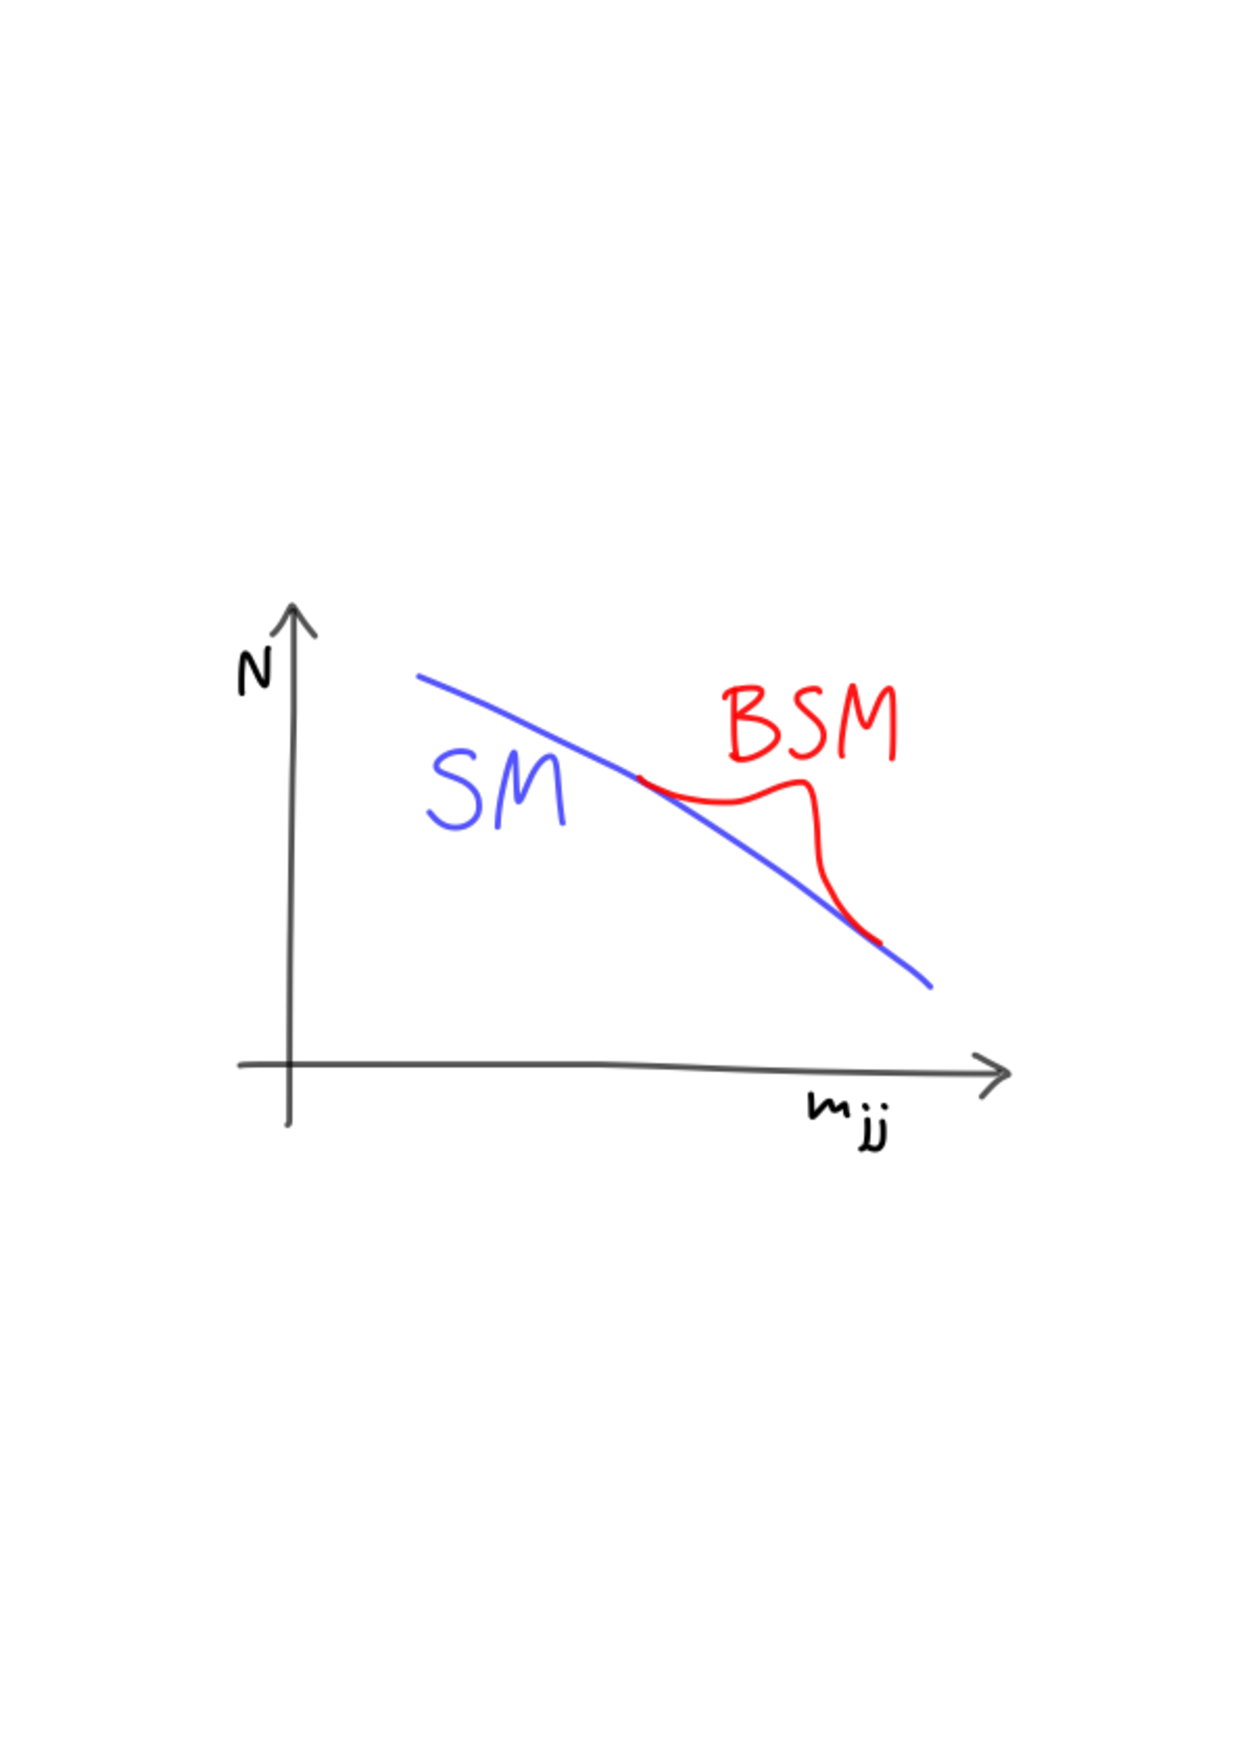
\includegraphics[width=0.65\linewidth, angle=0]{figs/Dibjet/Gen/dijet_schem.pdf}
  \end{center}
  \vspace{-3mm}
  \caption{A cartoon illustrating the use of the dijet invariant mass (\mjj) distribution in the search phase of the di-$b$-jet analysis.
            Shown is the smoothly falling distribution from multi-jet QCD (SM)
            and a resonance shape caused by a Beyond Standard Model particle (BSM)}
          \label{fig:evt-dijet_schem}
  \end{figure}
  \vspace{-4mm}
 
\item\textbf{Limit Setting:} (\textit{Chapter~\ref{sec:lim}})\\
  If, in the search phase stage of the analysis, no significant evidence of signal is
  found then some of the signal models considered may be excluded.
  95\% confidence level limits are set on the two benchmark signals considered.
  Chapter~\ref{sec:lim} presents the limit-setting methodology,
  a description of systematics considered
  and the limit results for each of the data-sets considered.

\end{itemize}

\section{List of Data Sets Used}
\label{sec:evt-datasets}

The di-$b$-jet analysis is performed in several iterations
as data is being collected, where each iteration uses a different data-set.
This is done for two reasons;
firstly it is important to know as soon as possible
if there is evidence of a new resonance as
this would affect the strategy of future di-$b$-jet analyses and that of other analyses at ATLAS.
Secondly, this allows us to incrementally
expand, adapt and improve this strategy in each iteration of the analysis.

In this thesis three different data-sets are considered by the di-$b$-jet analysis.
The overall analysis strategy is the same for each data-set,
so the iterations are described together.
However, there are some significant differences in the details;
as such during the analysis description it will be clearly labelled
which data-set is being referred to.

For any data-set a Good Run List (GRL)
is applied to remove events of low data-quality,
which is typically because an element of the detector was not operating optimally.
For example, data-taking periods where the inner-most layer of the inner detector,
the IBL, was not operating are removed as
this data-taking period has a lower $b$-tagging performance.
A GRL is applied to all data-sets considered in this analysis.

The data-sets are listed below, the trigger used in each data-set is described.
All quoted luminosities are given after the GRL has been applied.

\begin{itemize}[leftmargin=*]
\item\textbf{Summer16+15}: \\
  The \verb|Summer16+15| data-set contains 13 TeV $pp$ collision data collected
  between January 2015 to July 2016 which has an integrated luminosity 13.3~\ifb.
  The trigger used in this data-set, known as \verb|HLT_j380|,
  requires a trigger-level jet with $p_T >$ 380 GeV
  \footnote{\label{foot1} Further details of single-jet triggers is in Section~\ref{sec:trig-jet}.}.
  The analysis on this data-set has been published as a conference note~\cite{dibjet-ichep_conf}. \\
  
\item\textbf{Full16+15\_HighMass}:\\
  The \verb|Full16+15_HighMass| data-set contains 13 TeV $pp$ collision data collected
  between January 2015 to December 2016, which has an integrated luminosity of 36.1~\ifb.
  The trigger used in this data-set, known as \verb|HLT_j380|,
  requires a trigger-level jet with $p_T >$ 380 GeV
  \footnote{Again, see  Section~\ref{sec:trig-jet} for details on single-jet triggers.}.
  The analysis on this data-set has yet to be published.\\
  
\item\textbf{Full16\_LowMass}: \\
  The \verb|Full16_LowMass| data-set contains 13 TeV $pp$ collision data collected
  between January 2016 to December 2016, which has an integrated luminosity of 24.3~\ifb.
  The trigger used in this data-set is a double $b$-jet trigger 
  which requires two trigger-level jets with $p_T >$ 150 GeV and $p_T >$ 50 GeV
  where both jets have been $b$-tagged at the trigger level
  \footnote{Further details of $b$-jet triggers and this particular trigger used in this analysis is in Section~\ref{sec:trig-bjet}.}.
  The \verb|Full16_LowMass| data-set uses a $b$-jet trigger as the lower \pT~thresholds allow
  the analysis to probe a lower range of \mjj.
  This analysis does not include data from 2015 which was collected using a significantly different $b$-jet trigger configuration.
  The \verb|Full16_LowMass| data-set uses a $b$-jet trigger aware GRL which additionally
  removes periods of data where the $b$-jet trigger was performing in a sub-optimal way,
  the GRL is described in Section~\ref{sec:trig-grl}.
  As a double $b$-jet trigger is used only the 2 $b$-tag category is considered.
  The analysis on this data-set has yet to be published.

\end{itemize}

\section{Backgrounds and Signal}
\label{sec:evt-s+b}

In the di-$b$-jet analysis selection two
benchmark signal models and one dominant background are considered.
The signal models and dominant background are
used to optimise event selection, so I will describe
the signal and backgrounds considered here.

For both the background and the signal models Monte-Carlo simulation of the processes is produced.
Unless specified, the Monte-Carlo simulation is produced using
the \textsc{Pythia8}~\cite{dibjet-pythia8} program for event generation,
the \textsc{EvtGen} package~\cite{trig-evtGen} to model the decays of the $B$ and $C$ hadrons,
the A14 parameter set~\cite{dibjet-a14} to model the parton shower, hadronisation and underlying event,
and the NNPDF23LO PDF set~\cite{dibjet-nnpdf} to describe the Parton Distribution Function.
The detector response is modelled using the ATLAS detector simulation package~\cite{dijet-sim_ATLAS}.
%The effect of pile-up is modelled by superimposing simulated minimum-bias events
%on the hard-scatter simulation,
%where minimum-bias events are events collected with a loose trigger requirement
%and are dominated by inelastic scattering.

\begin{itemize}[leftmargin=*]
\item\textbf{Background: QCD Di-jet}:  \vspace{1em} \\
  Section~\ref{sec:theo-qcd} discussed the details of QCD dijet production.
  In particular in Section~\ref{sec:theo-qcd-dijet_features} it was noted that the
  relative strength of the strong force compared to other forces
  of the Standard Model means that
  QCD dijet production would dominate other backgrounds in a di-$b$-jet event selection.
  Hence, this will be considered as the only background.
  A description of how the QCD dijet background is modelled in this analysis is described in Chapter~\ref{sec:bkg}.
  A simulated QCD dijet sample is also used in this analysis
  for background studies and background modelling validation.
  \end{itemize}

\noindent
Before describing the signal models used it is useful to clearly differentiate between the two definitions of mass used in this analysis.
The invariant dijet mass or reconstructed mass is the invariant mass of the two leading jets, and is denoted by~\mjj.
The simulated mass is the true mass of particle causing a resonance and is defined at the generator level.
The two differ due to detector uncertainties when measuring jet energy.

\begin{itemize}[leftmargin=*]
\item\textbf{Signal: $Z'$ Boson}:  \vspace{1em} \\
  The $Z'$ boson is an additional gauge boson that can decay to two $b$-quarks,
  the theoretical $Z'$ boson models considered are
  described in detail in Section~\ref{sec:theo-bsm_zprime}.
  The $Z'$ boson provides a benchmark model in the 2 $b$-tag category.\\
  %in the case that both jets have been $b$-tagged.

  In the \verb|Summer16+15|, \verb|Full16+15_HighMass| and \verb|Full16_LowMass| data-set analyses
  the Sequential Standard Model (SSM) $Z'$ and the leptophobic $Z'$ models are considered.
  The intrinsic width of the $Z'$ boson has been set to 3\% of the simulated mass.
  Monte-Carlo simulation is used to produce \mjj~signal templates at leading order (LO).
  Only decays to $b\bar{b}$ are simulated;
  other decays of the  $Z'$ boson are ignored such that our
  results are easier to interpret for other signal models decaying to pairs of $b$-quarks.
  It has been shown that for a $Z'$-boson model the cross-sections can increase by up to 30\%
  from the addition of next-to-leading order (NLO) diagrams~\cite{evt-NLO_zprime}.
  Therefore the signal template normalisation is corrected to account for NLO effects,
  the correction factors have been derived by comparing
  the LO and NLO matrix calculations performed using the \textsc{MadGraph} generator~\cite{dibjet-madGraph}
  and are found to be between 1.2 and 1.3 depending on the signal mass.
  Simulated SSM and leptophobic $Z'$ boson templates are produced at simulated mass points of
  600, 800, 1000, 1250, 1500, 1750, 2000, 2500, 3000, 4000 and 5000 GeV.\\
  
  Further to this, for the \verb|Full16+15_HighMass| and \verb|Full16_LowMass| data-sets
  the Dark Matter mediator $Z'$ boson is also considered.
  For this model the $Z'$ boson signal generation is performed at next-to-leading order using the \textsc{MadGraph5\_aMC@NLO} generator~\cite{dibjet-madGraph_NLO},
  whilst all other aspects of event modelling, including parton shower and hadronisation, are performed using the configuration with \textsc{Pythia8} as described above.
  The coupling of the $Z'$ boson to the Dark Matter fermion ($g_{DM}$) is set to 1 and
  the mass of the Dark Matter fermion is 10 TeV,
  the large mass means that decays to the Dark Matter fermion are supressed.
  For the \verb|Full16_LowMass| data-set the coupling to quarks ($g_{SM}$) is set to 0.1,
  decays to $b$, $c$ and light flavour quarks are considered,
  and the simulated mass points are 600, 800 and 1000 GeV.
  This configuration is chosen to be consistent with recomendations in~\cite{theo_bsm-zprime_dm},
  and to be consistent with other dijet searches at ATLAS~\cite{dijet-mori16_paper}.
  For the \verb|Full16+15_HighMass| data-set the coupling to quarks ($g_{SM}$) is set to 0.25
  and the simulated mass points are 1250, 1500, 1750, 2000, 2500, 3000, 4000 and 5000~GeV.
  The larger $g_{SM}$ value is chosen as larger cross-sections are required to set limits at high mass.
  For the \verb|Full16+15_HighMass| data-set only decays to $b$-quarks are considered
  as this allows for a greater number of simulated $Z' \to b\bar{b}$ events
  \footnote{This is required as the signal acceptance is lower at high mass, which will be shown in Section~\ref{sec:evt-sel-acc}.}.\\
  
  %Similarly the same models are considered in the \verb|Full16+15_LowMass|... \\

\item\textbf{Signal: $b^*$ Quark}:  \vspace{1em} \\ 
  The $b^*$ quark is the third generation excited quark which results from
  quark compositeness models.
  The dominant decay mode of the  $b^*$ quark is to $bg$.
  The model considered is
  described in detail in Section~\ref{sec:theo-bsm_bstar}.
  The $b^*$ quark provides a benchmark model in the $\geq$1~$b$-tag category.\\
  %case that at least one of the jets has been $b$-tagged.
  
  In the \verb|Summer16+15| and \verb|Full16+15_HighMass|
  data-sets the same $b^*$ quark model is considered.
  Monte-Carlo simulation is used to produce a $b^*$ quark \mjj~signal template.
  Only leading order calculations are considered.
  %again \textsc{Pythia8}~\cite{dibjet-pythia8} with the A14~\cite{dibjet-a14} tune and the NNPDF23LO PDF set~\cite{dibjet-nnpdf} is used.
  Decays to $bg$, $b\gamma$, $bZ_0$ and $tW^{-}$ are considered.
  In the \verb|Full16+15_LowMass| data-set
  only the 2 $b$-tag category is used
  and as such that the $b^*$ quark model is not considered.
  %further details can be found in Section~\ref{sec:evt-sel-btag}.
  Simulated $b^*$ quark templates are produced at simulated mass points of
  1250, 1500, 1750, 2000, 2500, 3000, 4000 and 5000~GeV.
\end{itemize}

\section{Event Selection}
\label{sec:evt-sel}

The overall aim when designing the di-$b$-jet analysis event selection
is two-fold.
Firstly, events are selected to
maximise sensitivity to signal;
which is approximated in terms of $S$/$\sqrt{B}$,
where $S$ is the number of benchmark signal events and $B$ is the number of background events.
Secondly, the smoothly falling nature of the background needs to be maintained
as this is the underlying assumption of the background estimation strategy,
which will be described in Chapter~\ref{sec:bkg}.
In addition, it is desirable that the event selection for the
\verb|Full16+15_HighMass| and \verb|Full16_LowMass| data-set are
harmonised where possible such that the two analyses can be published together.
Any differences in event-selection between the two must be well motivated.

The di-$b$-jet event selection is split up into three sections each described separately.
Firstly, a pair of jets are selected (Section~\ref{sec:evt-sel-jets}),
then a set of event-level kinematic cuts are applied using the selected jets (Section~\ref{sec:evt-sel-event})
and finally $b$-tagging is applied to the jets (Section~\ref{sec:evt-sel-btag}).
In Section~\ref{sec:evt-sel-acc} the full event selection is summarised and
the signal acceptance is evaluated.

The event selection is slightly different for each of the data-sets considered,
these differences will be noted and discussed in the text.

\subsection{Jet Selection}
\label{sec:evt-sel-jets}

Jets are reconstructed using the anti-$k_T$ algorithm with $R=0.4$
and calibrated using the EM+JES scheme;
a full description of jets used in this analysis is in Section~\ref{sec:obj-jets}.

At least two jets are required in an event.
The two highest \pT~jets, referred to as the leading and subleading jet,
are the jets used throughout this analysis.
To reduce the number of fake jets from sources such as calorimeter noise
both jets are required to pass \textit{loose} jet cleaning cuts
based on the properties and distributions of the energy deposits in the calorimeter associated to the jet;
details can be found in~\cite{evt-jet_cleaning}.

Cuts are applied to the leading and subleading jet-\pT~such that events are on the trigger plateau;
the kinematic region where all events passing the offline jet-\pT~selection
would also pass the online jet-\pT~requirements of the trigger
\footnote{Online refers to reconstructed objects used in the trigger decision
  whilst offline refers to objects reconstructed after events have passed the trigger at the data-processing level,
  from the definition in Section~\ref{sec:trig-bjet_eff}.}.
The jet-\pT~above which which a single jet-trigger is on the trigger plateu is referred to as the threshold jet-\pT.

For the \verb|Summer16+15| data-set; it is required that the leading jet has \pT~$>$ 430 GeV to be on the trigger plateau of \verb|HLT_j380|.
This cut is derived by comparing the leading jet-\pT~distributions of jets that pass the trigger, \verb|HLT_j380|,
relative to a benchmark trigger with a lower jet-\pT~threshold, \verb|L1_J75|.
Figure~\ref{fig:evt-ICHEP_turnon}(a) shows this comparison in one run of data where \verb|L1_J75| was unprescaled
\footnote{Unprescaled means that the trigger accepts every event passing the trigger selection criteria};
in the ratio plot it is shown that for leading jet-\pT~$>$ 430 GeV events are on the trigger plateau.
The subleading jet is required to have jet-\pT~$>$ 60 GeV
to avoid contamination from pile-up jets
\footnote{Specifically, if jets have~\pT~$<$ 60 GeV then it is recommended that
  a pile-up suppression algorithm know as JVT is used~\cite{evt-jvt}.
  There is little gain in acceptance from the addition of low~\pT~subleading jets and
  complications from implementing the recommendations so the jets are removed. }.
Both jets  are required to have $|\eta| <$ 2.4
such that the jets lie within the volume of the ATLAS pixel detector,
which is essential for optimal $b$-tagging performance.

\begin{figure}[!ht]
  \begin{center}
    \captionsetup[subfigure]{aboveskip=0pt,justification=centering}
    \subcaptionbox{Jet-\pT~($p_T^{\text{lead}}$) } {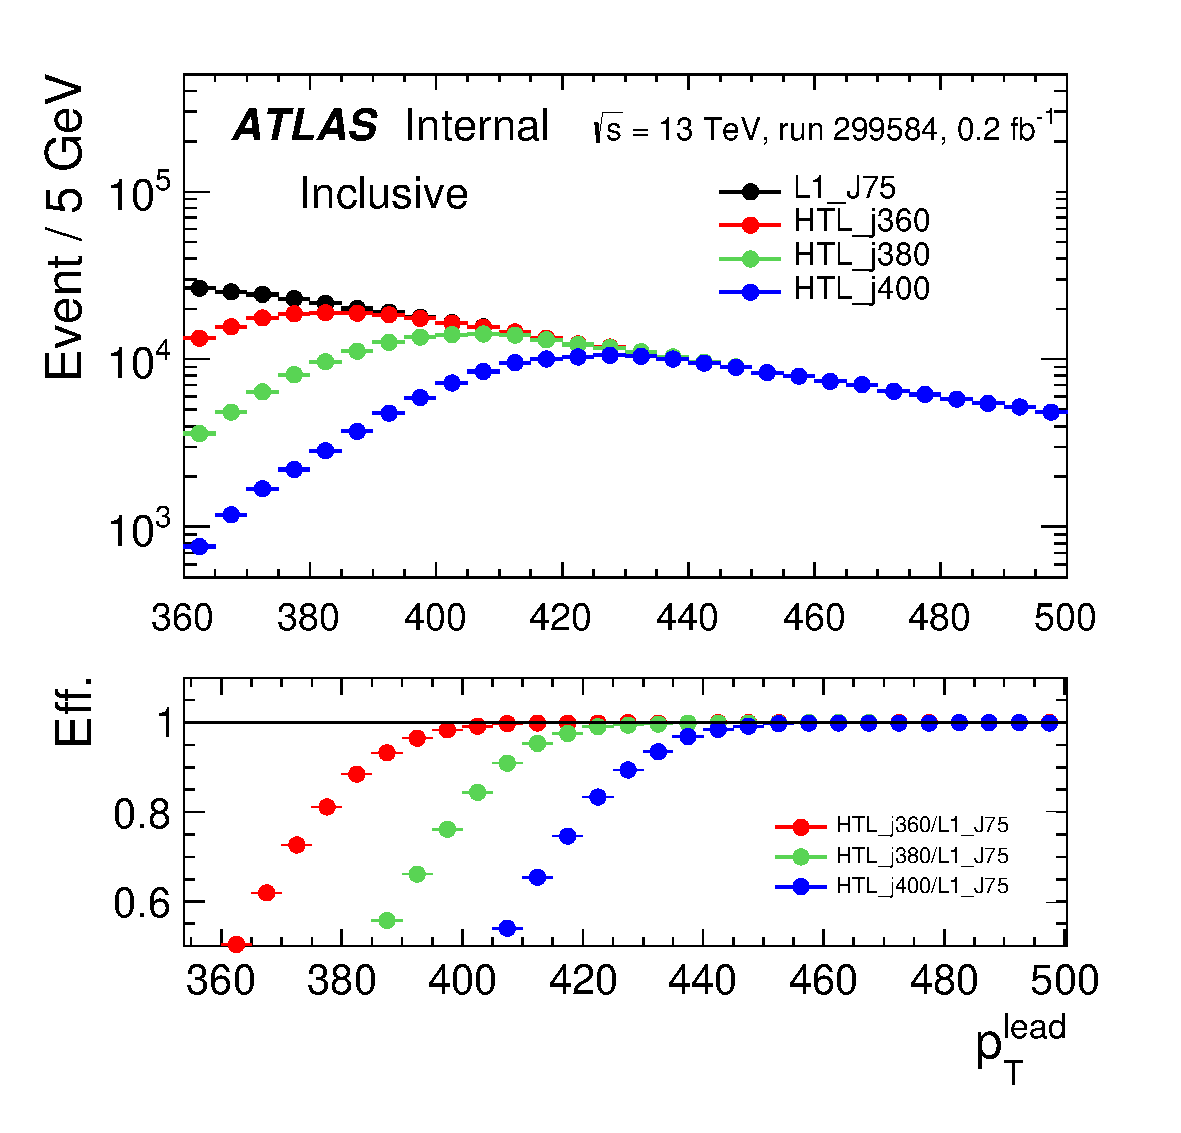
\includegraphics[width=0.45\linewidth, angle=0]{figs/Dibjet/ICHEP/evt-jet_pt.pdf}}
    \subcaptionbox{\mjj}                   {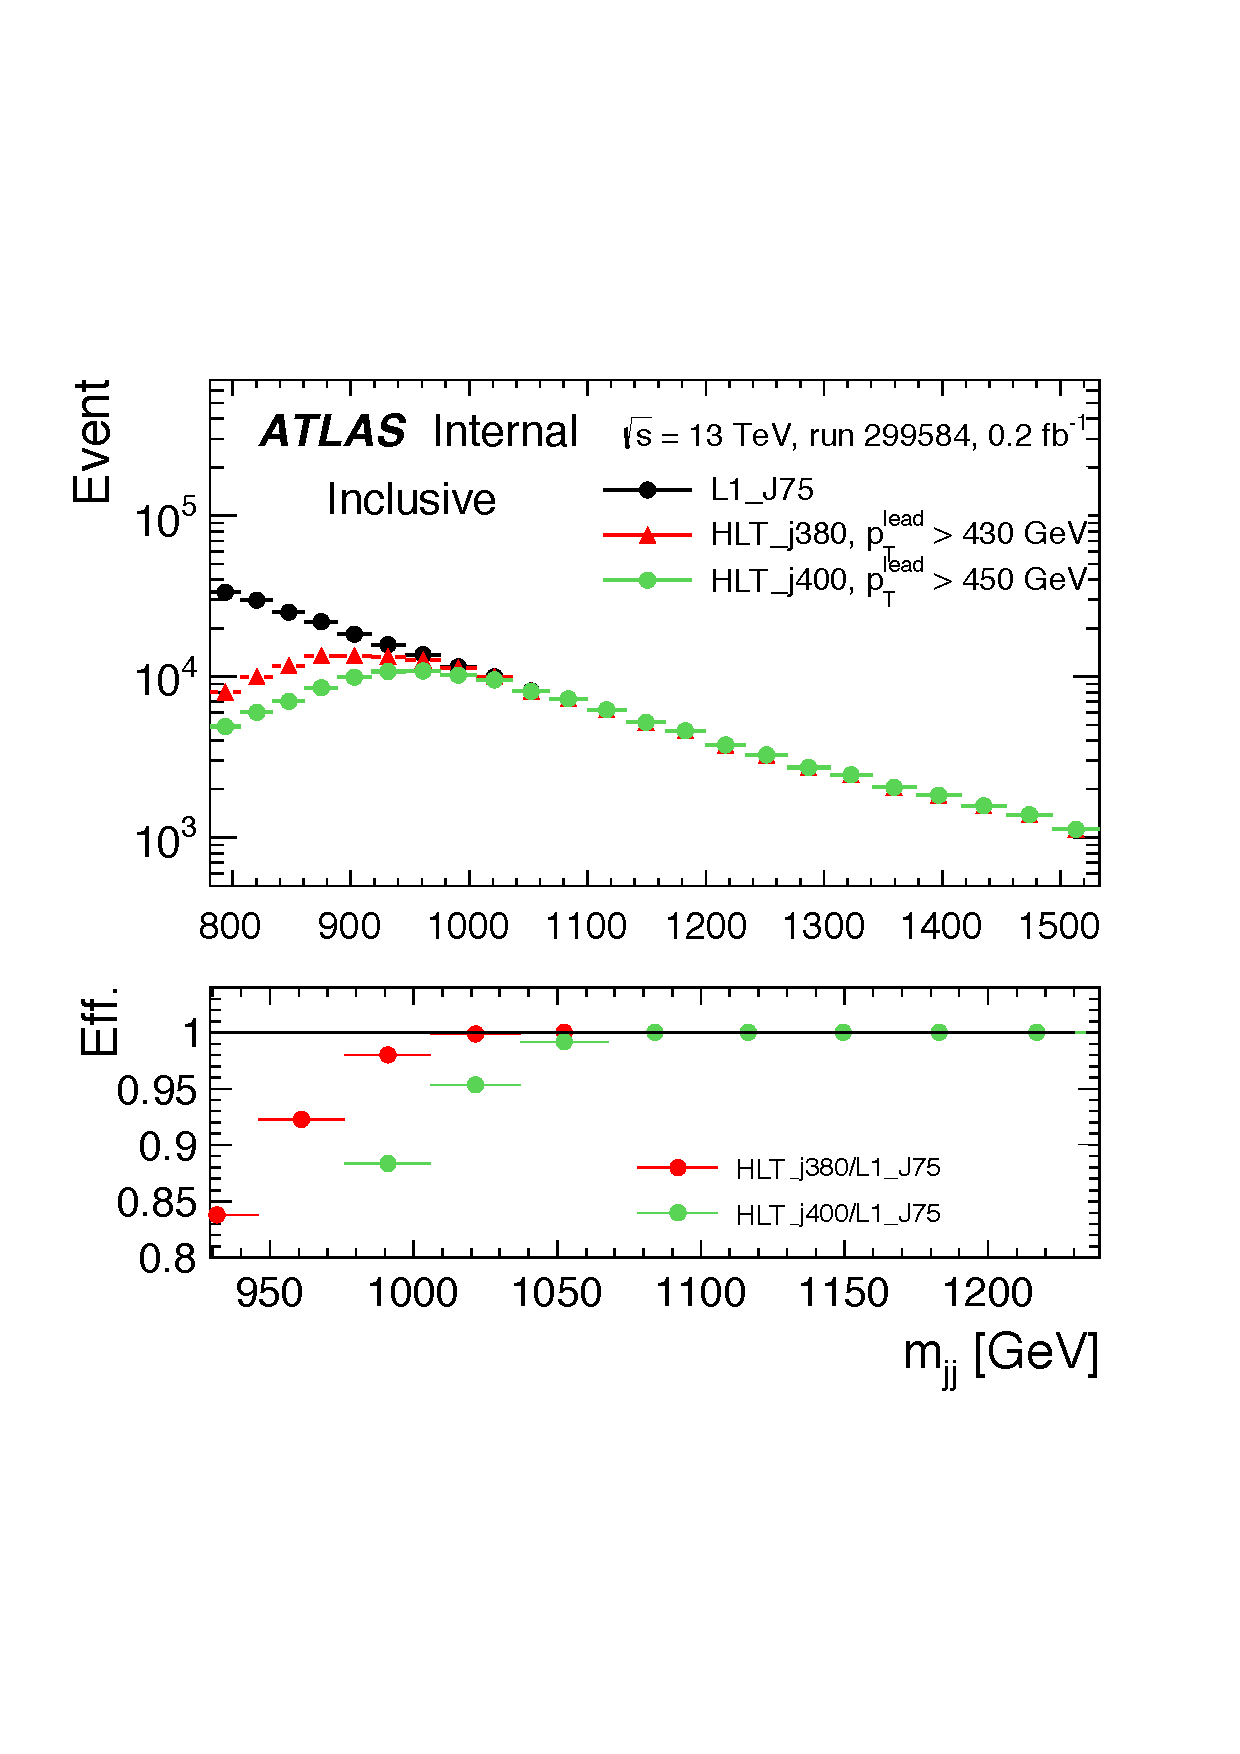
\includegraphics[width=0.44\linewidth, angle=0]{figs/Dibjet/ICHEP/evt-mjj.pdf}}
  \end{center}
  \caption[The comparisons of the (a) leading jet-\pT~($p_T^{\text{lead}}$) and (b)~\mjj~using events that passed an
            unprescaled L1\_J75 trigger (black) compared to events that pass a range of single-jet triggers (coloured) in one run of 2016 data.
            As shown in the legend, the single-jet triggers considered are HLT\_j380, HLT\_j400 and, in plot (a), HLT\_j360.
            In plot (b) the \textit{Summer16+15} event selection (excluding $b$-tagging) is applied with a leading jet-\pT~cut as described in the legend.
            The ratio with respect to L1\_J75 is shown in the lower panel.]
          {The comparisons of the (a) leading jet-\pT~($p_T^{\text{lead}}$) and (b)~\mjj~using events that passed an
            unprescaled L1\_J75 trigger (black) compared to events that pass a range of single-jet triggers (coloured) in one run of 2016 data.
            As shown in the legend, the single-jet triggers considered are HLT\_j380, HLT\_j400 and, in plot (a), HLT\_j360.
            In plot (b) the \textit{Summer16+15} event selection (excluding $b$-tagging) is applied with a leading jet-\pT~cut as described in the legend.
            The ratio with respect to L1\_J75 is shown in the lower panel~\cite{dibjet-ichep_conf}.}
     \label{fig:evt-ICHEP_turnon}
\end{figure}

For the \verb|Full16+15_HighMass| data-set the trigger \verb|HLT_j380| is also used,
and as such the leading jet is again required to have \pT~$>$ 430 GeV.
The subleading jet-\pT~is required to be $>$ 80 GeV to be consistent with the subleading jet-\pT~cut in the \verb|Full16_LowMass| event selection,
which will be described in the following paragraph.
Both jets  are required to have $|\eta| <$ 2.0;
the tighter cut on $|\eta|$ (relative to the \verb|Summer16+15| data-set) is selected
as at large values of jet-$|\eta|$ the $b$-Jet energy scale uncertainty is much larger.

For the \verb|Full16_LowMass| data-set a double $b$-jet trigger has been used;
which requires a trigger jet with $p_T >$ 150 GeV and a trigger jet with $p_T >$ 50 GeV.
To find the threshold jet-\pT~of the two single-jet triggers,
a linear fit to the threshold jet-\pT~of a range of single jet triggers is used,
details of the fit can be found in Appendix~\ref{app:triggerTurnOn_fit}.
Using the results of the fit the leading jet is required to have~\pT~$>$ 200 GeV
and the subleading jet is required to have~\pT~$>$ 80 GeV.
Both jets  are required to have $|\eta| <$ 2.0,
such that the $|\eta|$ cut is consistent for the \verb|Full16_LowMass| and \verb|Full16+15_HighMass| event selection.

%\begin{figure}[!ht]
%  \begin{center}
%    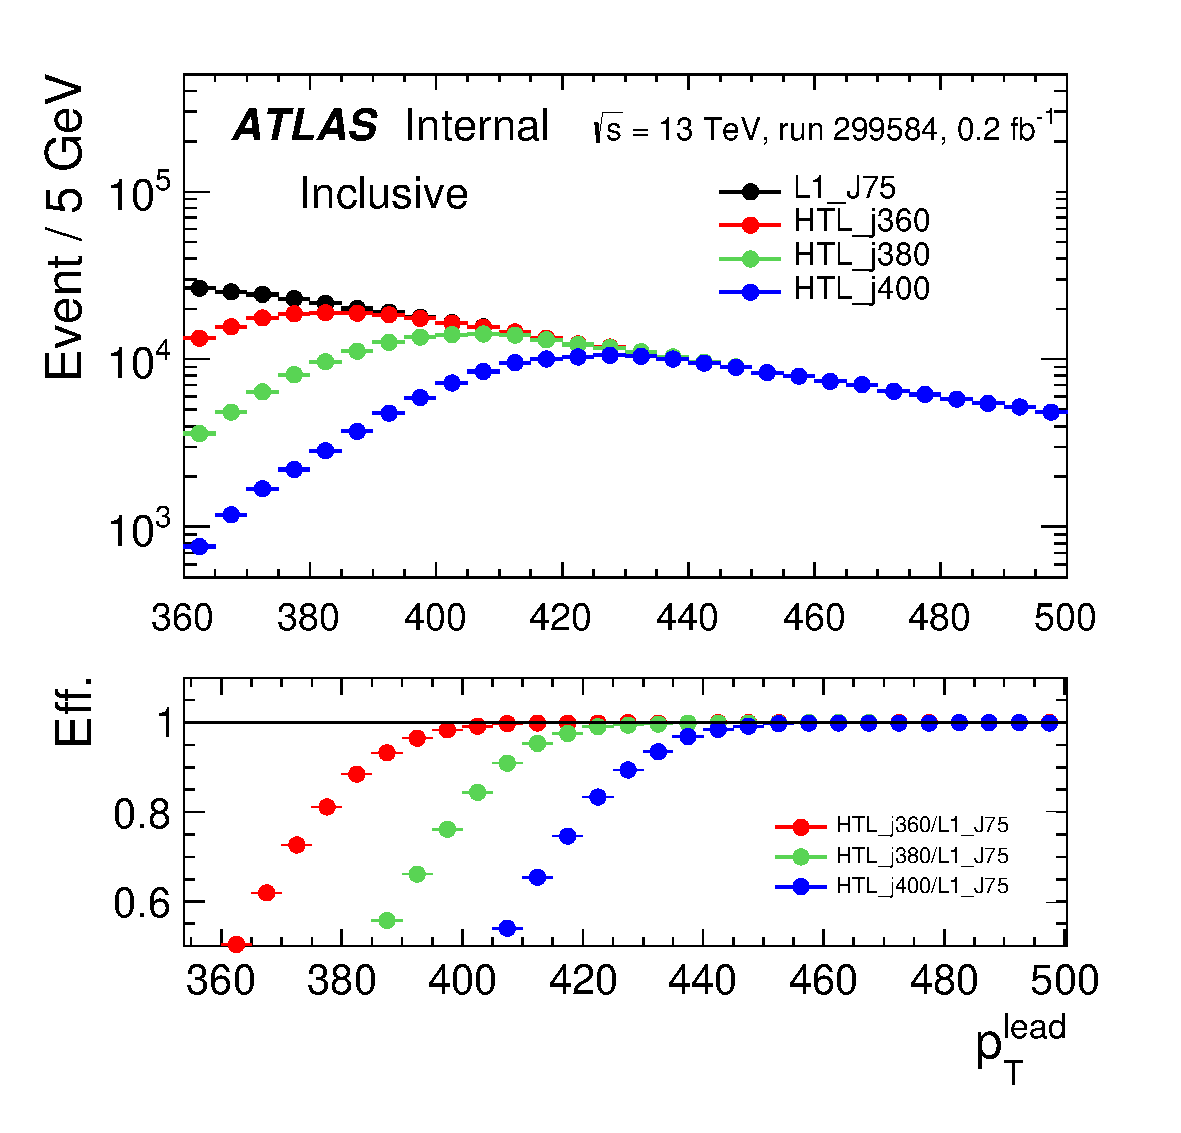
\includegraphics[width=0.8\linewidth, angle=0]{figs/Dibjet/ICHEP/evt-jet_pt.pdf}
%  \end{center}
%  \caption[The comparisons of the leading jet-\pT~using unprescaled L1\_J75 trigger (black dots) to the HLT\_J360 trigger (red dots),
%    HLT\_J380 trigger (green dots) and HLT\_J400 trigger (blue dots) in one run of 2016 data.
%  The ratio with respect to L1\_J75 is shown in the lower panel.]
%        {The comparisons of the leading jet-\pT~using an unprescaled L1\_J75 trigger (black dots) to the HLT\_J360 trigger (red dots),
%          HLT\_J380 trigger (green dots) and HLT\_J400 trigger (blue dots) in one run of 2016 data.
%          The ratio with respect to L1\_J75 is shown in the lower panel~\cite{dibjet-ichep_conf}.}
%  \label{fig:evt-jet_pt}
%\end{figure}

\subsection{Event Level Cuts}
\label{sec:evt-sel-event}

Using the two selected jets; there are a set of event-level requirements.
Firstly, events are required to have good reconstruction quality;
specifically the primary vertex
must have at least two tracks associated with it
and events with problematic reconstruction in the Tile calorimeter, LAr calorimeter or SCT are rejected.
\textbf{LM Fix, not sure what these are}

\noindent
Secondly, there is a cut applied to the variable $y^*$, defined as
\begin{equation}
  y^* = \frac{(y_1-y_2)}{2}
\end{equation}
where $y_1$ and $y_2$ are the rapidities of the leading and subleading jet respectively.
As discussed in Section~\ref{sec:theo-qcd-dijet_features}, QCD dijet production can occur through $t$-channel processes leading to more background events at large values of $|y^*|$,
whilst signal production occurs only through $s$-channel processes so will have no dependence on $y^*$.
Therefore, requiring $|y^*|$ below some threshold value will lead to an increased $S/\sqrt{B}$.

In the \verb|Summer16+15| data-set it is required that $|y^*| <$ 0.6.
This value has been shown to maximise $S/\sqrt{B}$ when no $b$-tagging is applied
at previous inclusive dijet searches at ATLAS~\cite{dijet-mori16_paper}
\footnote{Inclusive dijet analysis means a dijet analysis where no $b$-tagging is applied}.
The effect of $b$-tagging on the optimal value of this cut is assumed to be small,
as $t$-channel processes still dominate the background.

In the \verb|Full16+15_HighMass| data-set it is required that $|y^*| <$ 0.8.
This value is derived by calculating $S/\sqrt{B}$ in the 2 $b$-tag category for a range of simulated mass points
using the SSM $Z'$-boson model as signal and the QCD background from simulation as background.
It has been found that $|y^*| <$ 0.8 maximises $S/\sqrt{B}$.

In the \verb|Full16_LowMass| data-set it is required that $|y^*| <$ 0.6.
The $|y^*|$ cut was not harmonised with the \verb|Full16+15_HighMass| data-set
as it was shown that the looser cut introduced a kinematic bias at low values of~\mjj.
This will be demonstrated below.

Finally, the invariant mass of the two leading jets, \mjj, is required to be above a threshold value.
This cut ensures that there is no kinematic bias on the \mjj~distribution
from the trigger or jet-\pT~requirements described in Section~\ref{sec:evt-sel-jets}.
In addition, it is also required that the background is smooth in the \mjj~region chosen
such that it can be described using our background modelling strategy.

In the \verb|Summer16+15| data-set it is required that \mjj~\gt~1378 GeV;
which ensures the two conditions listed above are met.
Firstly, Figure~\ref{fig:evt-ICHEP_turnon}(b) shows the comparison of \mjj~distributions for events
that pass the \verb|Summer16+15| data-set event selection (exluding $b$-tagging), including the trigger \verb|HLT_j380|,
compared to events that pass a reference trigger, \verb|L1_J75|,
in one run of data where \verb|L1_J75| was unprescaled.
The ratio plot demonstrates that for \mjj~\gt~1100 GeV there is no kinematic bias from the trigger or event-selection.
%therefore we conclude that for \mjj~\gt~1378 GeV there is also no kinematic bias.
Secondly, it has been shown using simulated events that
\mjj~\gt~1378 GeV is required such that the \mjj~distribution from QCD dijet production
can be described by our background modelling strategy;
this study is presented in Section~\ref{sec:bkg-summer_range}.
Hence, \mjj~\gt~1378 GeV is the loosest cut that meets both of the conditions.

In the \verb|Full16+15_HighMass| data-set it is required that \mjj~\gt~1200 GeV in the 2 $b$-tag category and
\mjj~\gt~1341 GeV in the $\geq1$ $b$-tag category;
which again ensures the two conditions required are met.
Firstly, Figure~\ref{fig:evt-ICHEP_turnon}(b) shows the comparison of \mjj~distributions for events
that pass the \verb|Full16+15_HighMass| data-set event selection (excluding $b$-tagging), including the trigger \verb|HLT_j380|,
compared to events that pass a reference trigger, \verb|L1_J100|,
in one run of data where \verb|L1_J100| was unprescaled.
The ratio plot demonstrates that for \mjj~\gt~1200 GeV there is no kinematic bias from the trigger or event-selection.
Secondly, it has been shown during the fit studies that
in the $\geq1$ $b$-tag category a cut of \mjj~\gt~1341 GeV is required such that the
\mjj~distribution from the background can be described by our background modelling strategy;
this study is presented in Section~\ref{sec:bkg-hm_spsig_1b}.
No such effect was observed in the 2 $b$-tag category.
Hence, \mjj~\gt~1200 GeV is required in the 2 $b$-tag category and
\mjj~\gt~1341 GeV is required in the 1 $b$-tag category.

%\begin{figure}[!ht]
%  \begin{center}
%    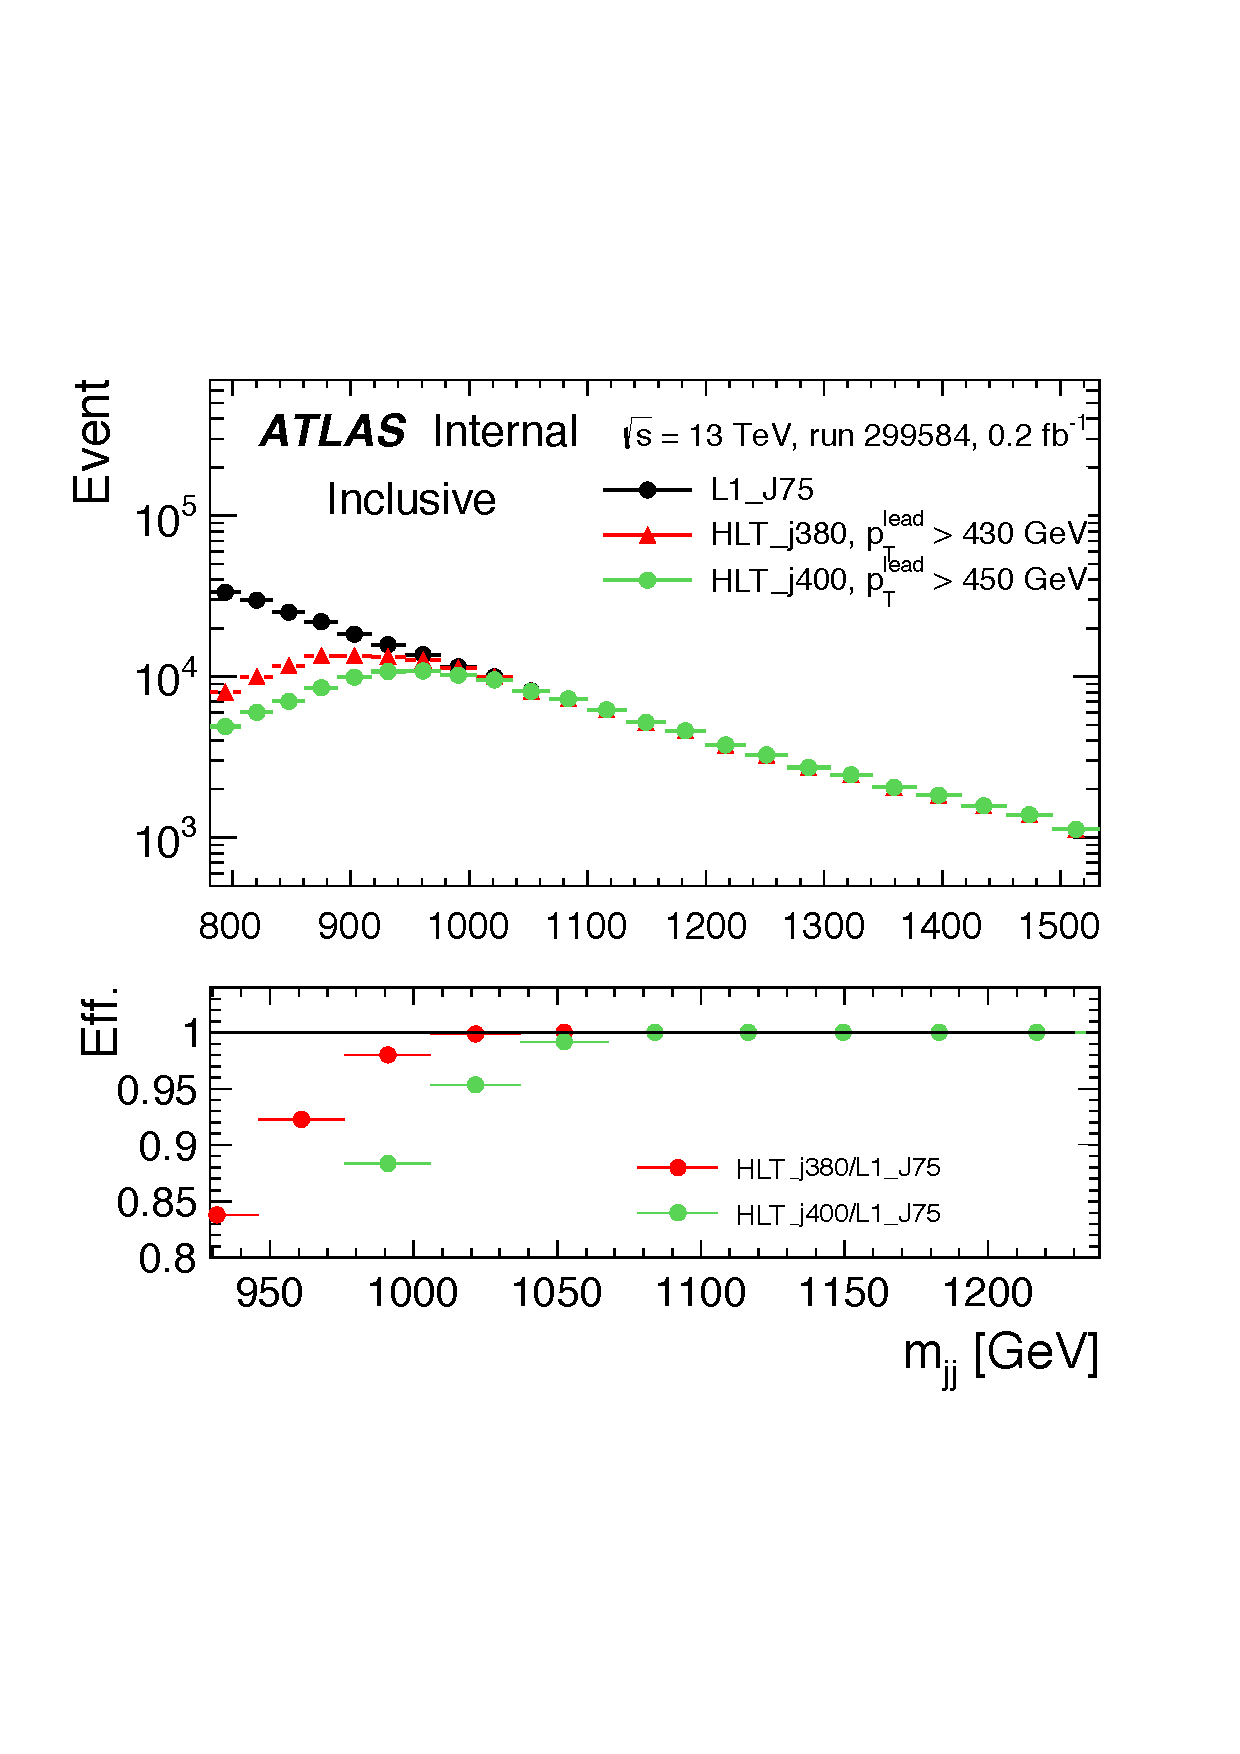
\includegraphics[width=0.8\linewidth, angle=0]{figs/Dibjet/ICHEP/evt-mjj.pdf}
%  \end{center}
%  \caption[The comparisons of the \mjj~distribution of events that pass an unprescaled L1\_J75 trigger (black dots) to the
%    events that pass the HLT\_J380 trigger with leading jet-\pT~\gt~430 GeV (red dots) and 
%    the HLT\_J400 trigger with a leading jet-\pT~\gt~450 GeV (green dots) in one run of 2016 data.
%    The ratio with respect to L1\_J75 is shown in the lower panel.]
%        {The comparisons of the \mjj~distribution of events that pass an unprescaled L1\_J75 trigger (black dots) to the
%    events that pass the HLT\_J380 trigger with leading jet-\pT~\gt~430 GeV (red dots) and 
%    the HLT\_J400 trigger with a leading jet-\pT~\gt~450 GeV (green dots) in one run of 2016 data.
%    The ratio with respect to L1\_J75 is shown in the lower panel~\cite{dibjet-ichep_conf}.}
%  \label{fig:evt-mjj}
%\end{figure}

For the \verb|Full16_LowMass| it is shown that for \mjj~\gt~500 GeV there is no kinematic bias
from the jet-\pT~cuts used in the \verb|Full16_LowMass| data-set event selection.
Figure~\ref{fig:evt-lowmass_turnon}(a) compares the~\mjj~distribution of events
that pass the event selection requirements that the leading (subleading) jet-\pT~$>$ 200 (80) GeV, labelled as `analysis~cuts',
compared to events that pass some arbitarily low cuts of leading (subleading) jet-\pT~$>$ 150 (50) GeV, labelled as `low~cuts'.
Events are required to pass the \verb|L1_J75| trigger and are taken from a run of 2016 data where \verb|L1_J75| was unprescaled.
The events are additionally required to pass the jet-$\eta$ and $y^*$ requirements of the \verb|Full16_LowMass| data-set event selection.
For \mjj~\gt~500 GeV there is no kinematic bias from the the \verb|Full16_LowMass| event selection,
this includes a one~\mjj~bin buffer that is used as a safety measure.
Figure~\ref{fig:evt-lowmass_turnon}(b) compares the~\mjj~distribution using the events that pass the analysis cuts and low cuts as before,
except that now a $|y^*| <$ 0.8 is applied.
For $|y^*| <$ 0.8 there is a kinematic bias in the~\mjj~range 500-544 GeV,
and as such the $|y^*| <$ 0.8 is not selected.

However, for the the \verb|Full16_LowMass|
there is an additional kinematic bias on~\mjj~
due to the effect of jets outside of the leading or subleading jet
that was discovered as the analysis progressed.
As a result the~\mjj~is required to be greater than 566 GeV.
To describe this effect I must first introduce $b$-tagging so
the studies and conclusion are described below in Section~\ref{sec:evt-set_btrigMatch}.

\begin{figure}[!ht]
  \begin{center}
    \captionsetup[subfigure]{aboveskip=0pt,justification=centering}
    \subcaptionbox{$|y^*| <$ 0.6} {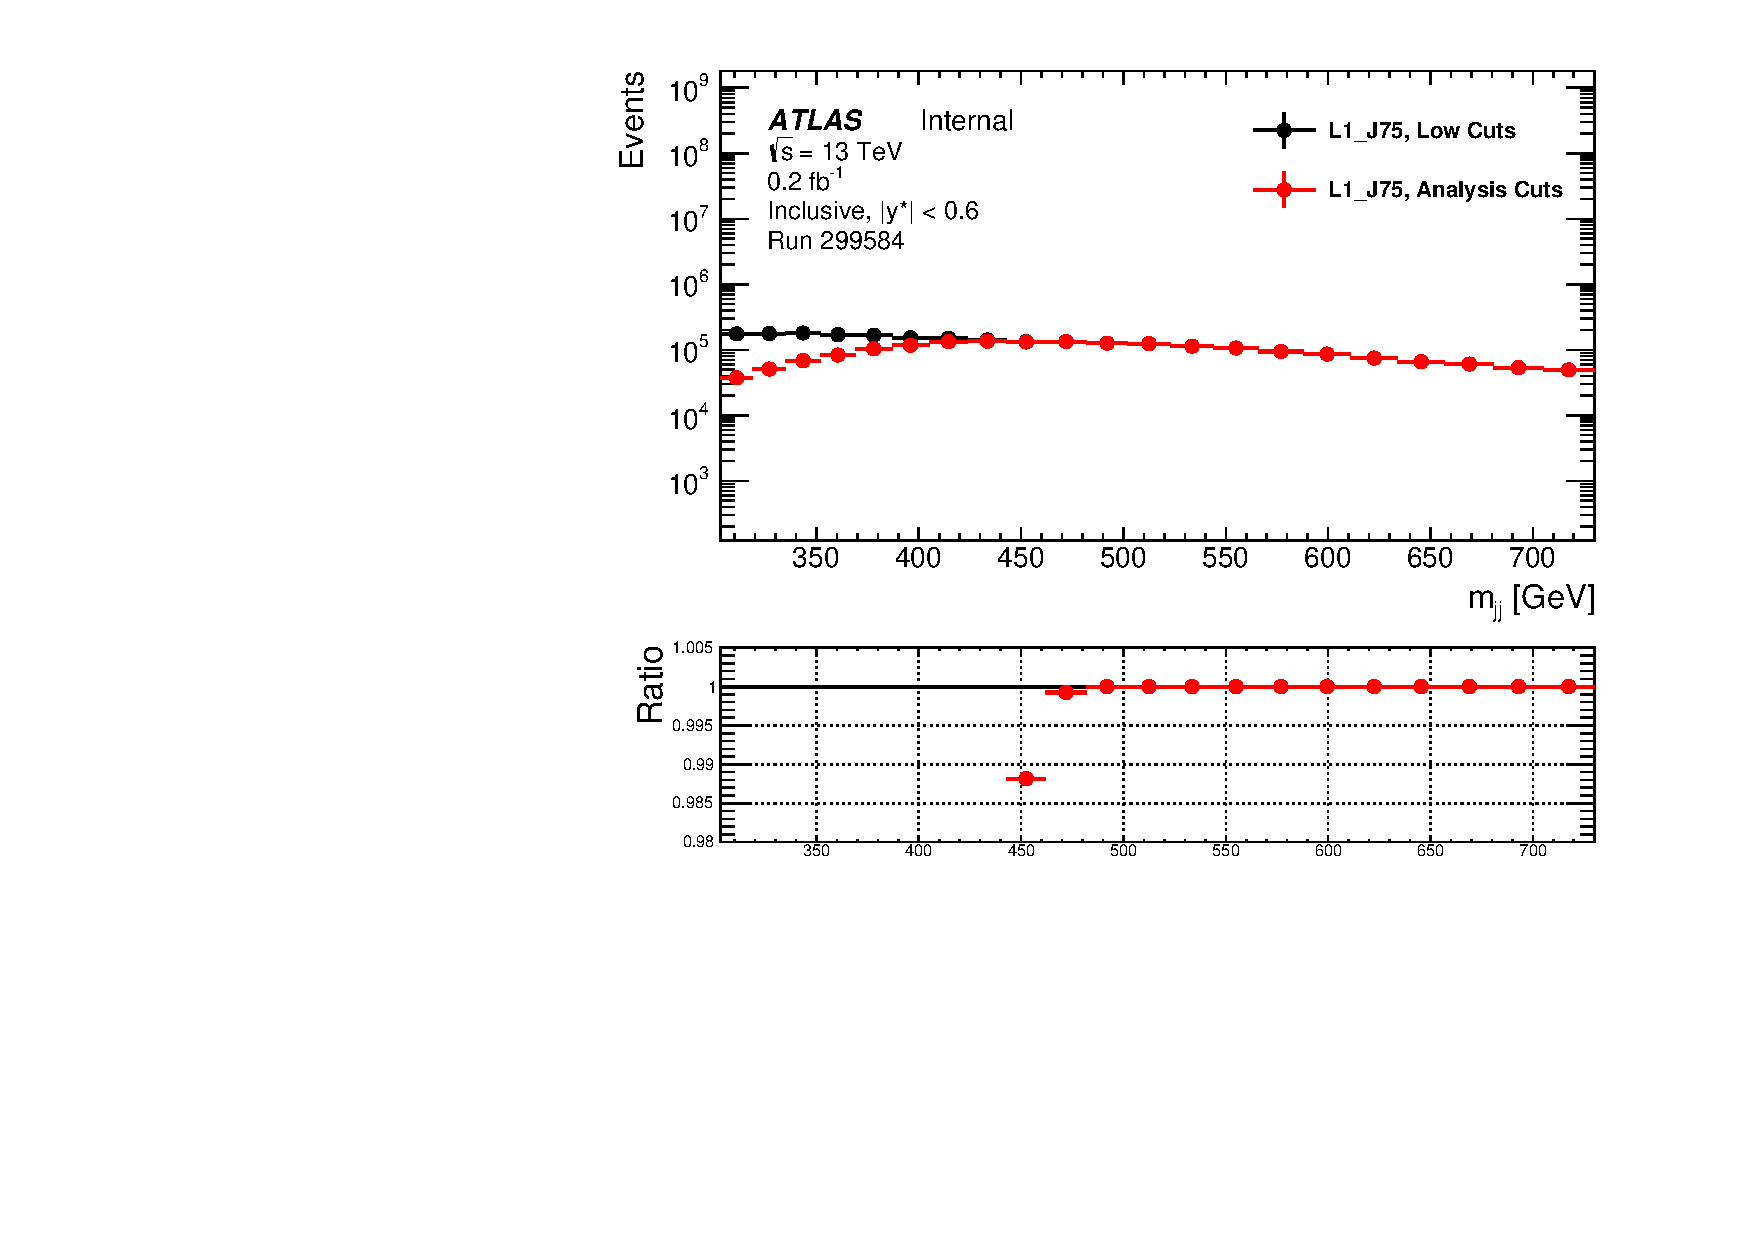
\includegraphics[width=0.48\linewidth, angle=0]{figs/Dibjet/LowMass/evt-mjj_yStar0p6.pdf}}
    \subcaptionbox{$|y^*| <$ 0.8} {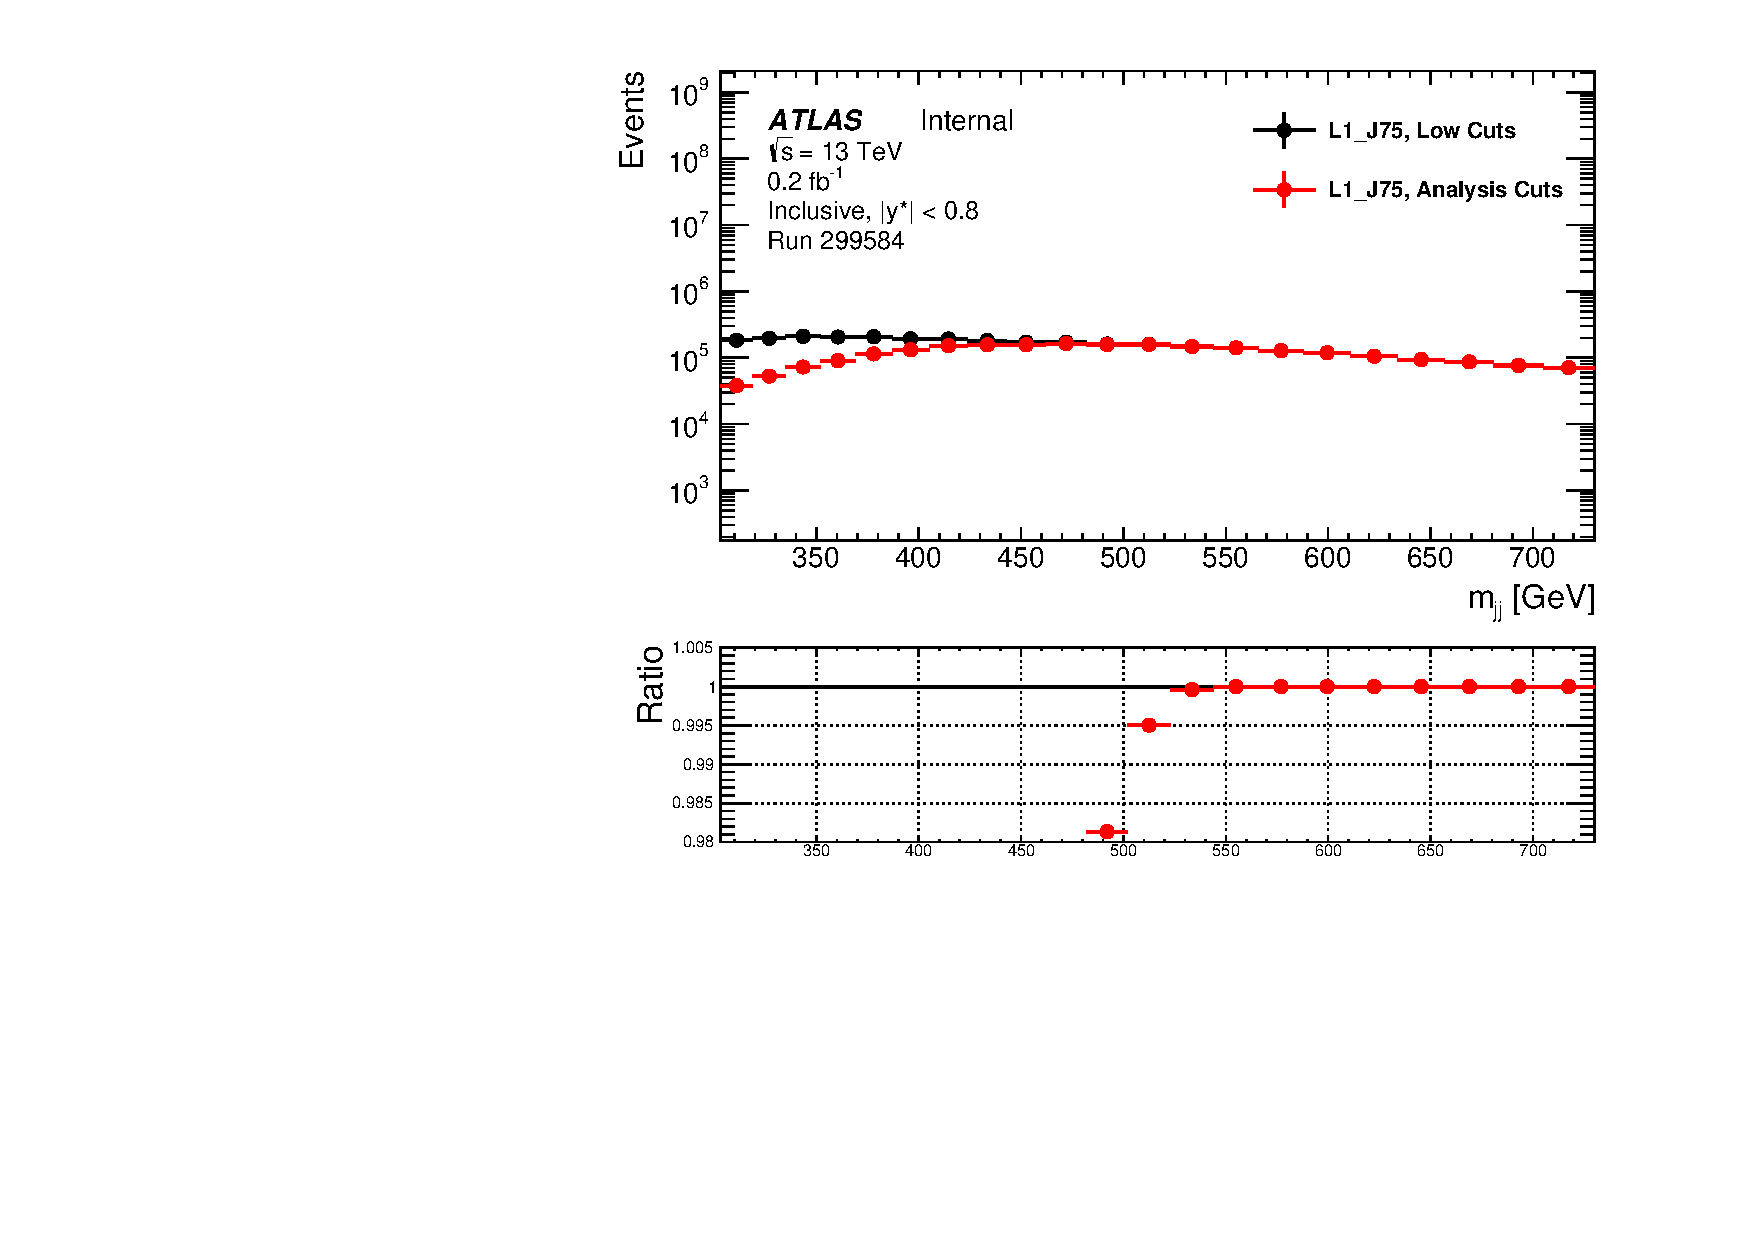
\includegraphics[width=0.48\linewidth, angle=0]{figs/Dibjet/LowMass/evt-mjj_yStar0p8.pdf}}
  \end{center}
  \caption{The comparisons of the~\mjj~of events that pass the analysis jet-\pT~cuts of leading (subleading) jet-\pT~$>$ 200 (80) GeV (black)
    compared to events that pass a set of low jet-\pT~cuts of leading (subleading) jet-\pT~$>$ 200 (80) GeV (red).
    The events are required to pass the L1\_J75 trigger and are taken from one run of 2016 data where the trigger L1\_J75 is unprescaled.
    In addition the events are required to have (a) $|y^*| <$ 0.6 and (b) $|y^*| <$ 0.6.
    No $b$-tagging cuts have been applied.}
     \label{fig:evt-lowmass_turnon}
\end{figure}

\subsection{$b$-Tagging}
\label{sec:evt-sel-btag}

The selection of $b$-jets, known as $b$-tagging,
forms an essential technique in the di-$b$-jet event selection.
A detailed description of $b$-tagging is found in Section~\ref{sec:obj-bjets}.
$b$-tagging is performed using a multi-variate algorithm known as MV2c10 which has been described in~\ref{sec:obj-bjets_MV2}.

Two $b$-tagging categories are used for the two different types of signal model considered.
The 2 $b$-tag category requires that both jets are $b$-tagged,
and is used to search for resonances decaying to 2 $b$-quarks such as the $Z'$ boson.
The $\geq 1$ $b$-tag category requires that at least one jet is tagged,
and is used to search for resonances decaying to 1 $b$-quark and a quark/gluon such as the $b^*$ quark.
The exclusive 1 $b$-tag category was also considered but was found to be less sensitive to the $b^*$ quark model.

In the \verb|Summer16+15| and \verb|Full16+15_HighMass| data-sets
$b$-tagging is performed using the 85\% operating point of the MV2c10 algorithm,
details on the operating points of MV2c10 are found in Section~\ref{sec:obj-bjets_MV2}.
This operating point was chosen to maximise $S/\sqrt{B}$ for a range of simulated mass points in the 2 $b$-tag category.

Below the details of the $b$-tagging optimisation study for the \verb|Full16+15_HighMass| data-set are shown,
the results also validate the choice of $b$-tagging operating point in the \verb|Summer16+15| data-set.
The number of background events, $B$, is estimated in
a narrow~\mjj~window around
each simulated mass point considered using a
18.9~\ifb~subset of data for the 2 $b$-tag category.
The number of signal events, $S$, is estimated
in the same narrow~\mjj~windows using 
the simulated SSM $Z'$-boson signal template
described in Section~\ref{sec:evt-s+b} scaled to 18.9~\ifb~\footnote{This is
  the amount of data collected when the studies where performed}.
The full \verb|Full16+15_HighMass| event selection has been applied.
Table~\ref{tab:evt-btag_hm} summarises $S/\sqrt{B}$ for each operating point;
the 85\% operating point is selected as it performs well across the full range of mass points considered.
The conclusions of this study are luminosity independent
as $S/\sqrt{B} \propto 1/\sqrt{L}$ such that the relative sensitivity
between operating points will be the same for all luminosities.

\begin{table}[ht]
\begin{center}
\begin{tabular}{|c||c|c|c|}
  \hline
  Simulated Mass [GeV]        &  1500  &   2000  &  2500  \\
  \hline
  Mass window [GeV]               & 1378-1573       &  1785-2114   &  2267-2659 \\
  \hline
  $S/\sqrt{B}$ for 85\% OP        &  2.02           &  0.72        &  0.21          \\
  $S/\sqrt{B}$ for 77\% OP        &  2.12           &  0.64        &  0.17          \\
  $S/\sqrt{B}$ for 70\% OP        &  1.73           &  0.47        &  0.12          \\
  $S/\sqrt{B}$ for 60\% OP        &  0.96           &  0.21        &  0.07          \\ \hline
\end{tabular}
\caption[The estimated $S/\sqrt{B}$ at 18.9~\ifb~for 4 different MV2c10 operating points (OP).
  $S$ is estimated using a SSM $Z'$-boson and $B$ is estimated using a 18.9~\ifb~subset of 2 $b$-tag category data.
  The \textit{Full16+15\_HighMass} data-set event selection has been applied.
  Three different simulated mass points are considered and the mass windows used
  to estimate $S$ and $B$ for each mass point are shown in the table.]
        {The estimated $S/\sqrt{B}$ at 18.9~\ifb~for 4 different MV2c10 operating points (OP).
  $S$ is estimated using a SSM $Z'$-boson and $B$ is estimated using a 18.9~\ifb~subset of 2 $b$-tag category data.
  The \textit{Full16+15\_HighMass} data-set event selection has been applied.
  Three different simulated mass points are considered and the mass windows used
  to estimate $S$ and $B$ for each mass point are shown in the table~\cite{dibjet-ichep_int}.}
\vspace{-2em}
\label{tab:evt-btag_hm}
\end{center}
\end{table}

To further understand the effect of $b$-tagging in this analysis the flavour composition of the background is studied.
The dijet flavour composition is defined as the truth flavour of both of the jets used in the di-$b$-jet analysis,
using the definition of truth flavour from Section~\ref{sec:obj-bjets_label}.
Figure~\ref{fig:evt-summer_flavcomp} shows the dijet flavour composition of the simulated QCD dijet background in
the case where no $b$-tagging has been applied (inclusive) and in the $\geq1$ and 2 $b$-tag categories.
For this figure the \verb|Summer16+15| data-set event selection has been applied,
although the distributions are very similar for the \verb|Full16+15_HighMass| data-set
as the same $b$-tagging operating point has been chosen.

\begin{figure}[!ht]
  \begin{center}
    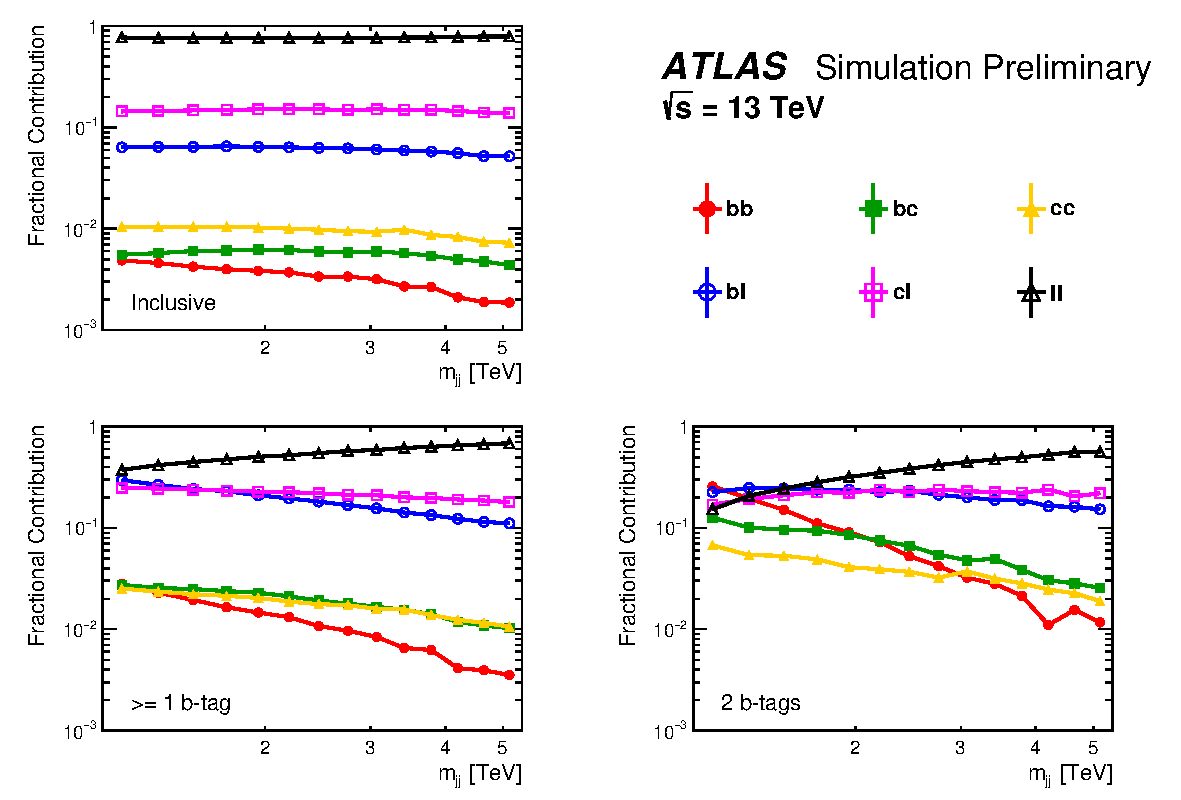
\includegraphics[width=0.99\linewidth, angle=0]{figs/Dibjet/ICHEP/evt-summer_flavcomp.pdf}
  \end{center}
  \caption{The dijet flavour composition of the simulated dijet background as a function of dijet mass,
    shown without applying $b$-tagging (inclusive) and for $\geq1$ $b$-tag and 2 $b$-tag categories.
    In the legend b, c and l refer to a truth matched $b$-jet, $c$-jet and light jet respectively.
    The \textit{Summer16+15} data-set event selection has been applied.}
  \label{fig:evt-summer_flavcomp}
\end{figure}

There are a few features that can be noted in this figure.
Firstly, the flavour fraction of the background before $b$-tagging is dominated by light-jets
for the reasons outlined in~Section~\ref{sec:theo-qcd-dijet_features}.
As the background is dominated by light-jets the application
of $b$-tagging can increase background rejection
and thus increase sensitivity to signal models that decay to $b$-quarks.
This motivates the use of $b$-tagging in the analysis.

Secondly, even after the application of $b$-tagging the largest contribution to the background is from light jets,
except for in a small region at low mass in the 2 $b$-tag category.
This shows that the sensitivity of the analysis is limited by the
light-jet rejection of $b$-tagging at high jet-\pT.

Finally, in all three cases the dijet flavour fractions are smooth, which is evidence that
there are no sudden changes in $b$-tagging efficiency of the background that could introduce
a non-smooth feature in the background invariant mass spectra.

\subsection{Effect of $b$-Trigger Matching in the \textit{Full16\_LowMass} Data-set}

In Section~\ref{sec:evt-sel-event} it was shown that for the \verb|Full16_LowMass| data-set
for~\mjj~\gt~500 GeV there is no kinematic bias in the~\mjj~distribution
due to the leading and subleading jet~\pT cuts.

However, it is also possible that jets other than the leading or subleading jet could fire the $b$-jet trigger.
I will refer to jets that are not the leading or subleading jet as `non-leading jets'.
To determine if non-leading jets are firing the $b$-jet trigger and what the size of the effect,
a study with trigger matching is considered.

Trigger matching is defined as requiring that the
leading and subleading jet must match to a trigger jet that passes the trigger level requirements.
An offline jet is matched to an online jet if $\Delta R$ between the jets $<$ 0.4.
The matching is exclusive, which means that no online or offline jet can be involved in two matchings.
If two matching are possible then the pair of jets with the smallest value of $\Delta R$ is chosen.

Once each offline jet is matched to an online jet then it can be required that
the leading and subleading jet must have online jets matched to them
and that the matched online jets must pass the double $b$-jet trigger requirements.
To be specific the trigger requirements are that
one online jet must have~\pT~\gt~150 GeV,
the other online jet must have~\pT~\gt~50 GeV
and that both jets must be $b$-tagged at the online 60\% operating point
\footnote{Further details of $b$-jet triggers and this particular trigger used in this analysis is in Section~\ref{sec:trig-bjet}.}..
I will refer to events that pass this requirement as `$b$-jet trigger matched' events.

In the ATLAS collaboration data is stored in objects know as `Derivations'
Each derivation contains only the events and the event information required to perform an analysis,
such that the data can be stored in a managable sized file.
For the di-$b$-jet analysis a derivation called EXOT2 is used
but, unfortunately, the trigger-level jet information is not present in EXOT2 derivation,
which is required to apply $b$-jet trigger matching.
Instead a derivation called FTAG2 is used, in which the trigger level information is present.
However, in FTAG2 not all events that pass the double $b$-jet trigger are not present.
In neither derivation is the full information required to do $b$-jet trigger matching on the full \verb|Full16\_LowMass| present.

To overcome this problem the effect of $b$-trigger matching can be estimated using the FTAG2 derivation.
Firstly, one can consider the~\mjj~spectrum of all events that pass the double $b$-jet trigger in
one period of data-taking which contains ...\ifb  of 2016 data-taking and
are included in the FTAG2 derivation when no $b$-jet trigger matching is applied.
I will refer to this as the~\mjj~spectrum from FTAG2
The full \verb|Full16_LowMass| data-set event selection has been applied to both.
Figure~\ref{evt-btrig_match}(a) shows this~\mjj~spectrum from FTAG2
compared to the~\mjj~spectrum equivalent using EXOT2, where all events are present,
the lower panel shows a ratio between the two.
One can notice that there is a deficit of events at low~\mjj.

Then the~\mjj~spectrum from FTAG2 described above can be compared to the~\mjj~spectrum of
all $b$-jet trigger matched events that pass the double $b$-jet trigger from the same Period of data.
The full \verb|Full16\_LowMass| data-set selection is applied.
Figure~\ref{evt-btrig_match}(b) shows the comparison of the two~\mjj spectra.
The lower panel shows the ratio between the two.

In the ratio plot of Figure~\ref{evt-btrig_match}(b) it is show that $\sim$ 5\% of events that
pass the \verb|Full16\_LowMass| event selection will not pass $b$-jet trigger matching.
In these cases a non-leading jet has fired that $b$-jet trigger.
For~\mjj~\gt~566 GeV this effect is smooth with respect to~\mjj~showing
that the effect of the non-leading jet will not cause a kinematic bias in this region.
In the region~\mjj~\lt~566 GeV there is a clear non-smoothness in the ratio plot,
which indicates that a kinematic bias could be present in the final data-set.

It is concluded that for~\mjj~\gt 566 GeV there is no evidence that
the effect of non-leading jets firing the double $b$-jet trigger
will cause a bias in the final data-set.
Therefore, for the \verb|Full16_LowMass| data-set it is required that~\mjj~\gt 566 GeV.

Finally it should be noted that for the 2017 reprocessing of data
the full information required for $b$-jet trigger matching is included in the EXOT2 dervation,
such that future iterations of the di-$b$-jet analysis can apply $b$-jet trigger matching.

\subsection{Event Selection Summary}
\label{sec:evt-sel-acc}

A summary of the  key components of the di-$b$-jet event selection
for each of the data-sets considered
is listed in Table~\ref{tab:evt}.

\begin{table}[!htb]
  \begin{tabular}{|c||c|c|c|}
    \hline
\thead{Cut}              &  \thead{Summer16+15} & \thead{Full16+15\_HighMass} & \thead{Full16+15\_LowMass} \\
\hline
%Trigger          & HLT\_380 & HLT\_380 & \makecell{ HLT\_j150\_bmv2c2060\_split\\\_j50\_bmv2c2060\_split} \\
Trigger                & Single-jet       & Single-jet    & Double $b$-jet (60\% OP) \\
Online LJ~\pT          & \gt~380 GeV      & \gt~380 GeV   & \gt~150 GeV  \\
Online SLJ~\pT         & -                & -             & \gt~50 GeV \\
\hline
Leading Jet-\pT    &  \gt~430 GeV & \gt~430 GeV &  \gt~200~GeV\\
Subleading Jet-\pT &  \gt~60 GeV & \gt~80 GeV  &  \gt~80~GeV\\
Jet-$|\eta|$   & $<$ 2.4 & $<$ 2.0 & $<$ 2.0 \\
\hline
$m_{jj}$  & \gt~1378 GeV & \makecell{\gt~1200 GeV (2 $b$-tag)\\ \gt~1341 GeV ($\geq1$ $b$-tag)} & \gt~500 GeV \\
$|y^*|$  & $<$ 0.6 & $<$ 0.8 & $<$ 0.6  \\
\hline
$b$-Tagging OP & 85\% & 85\% & 70\%\\
$b$-Tag Categories & 2 and $\geq$1 & 2 and $\geq$1 & 2 \\
\hline
\end{tabular}
\centering
\caption{A summary of the key event selections applied in the di-$b$-jet analysis for each of the data-sets considered.
For full details refer to the text.}
\label{tab:evt}
\end{table}

To better visualise events that pass the event selection,
Figure~\ref{fig:evt-vp1} show events displays for high~\mjj~events that pass
the $\geq$1 and 2 $b$-tag event selection respectively.
The figure was made using the VP1 event display package~\cite{evt-vp1}.
These events pass both the \verb|Summer16+15| and \verb|Full16+15_HighMass| data-set event selection.

\begin{figure}[!ht]
  \begin{center}
    \captionsetup[subfigure]{aboveskip=0pt,justification=centering}
    \subcaptionbox{2 $b$-tag\vspace{5mm}}      {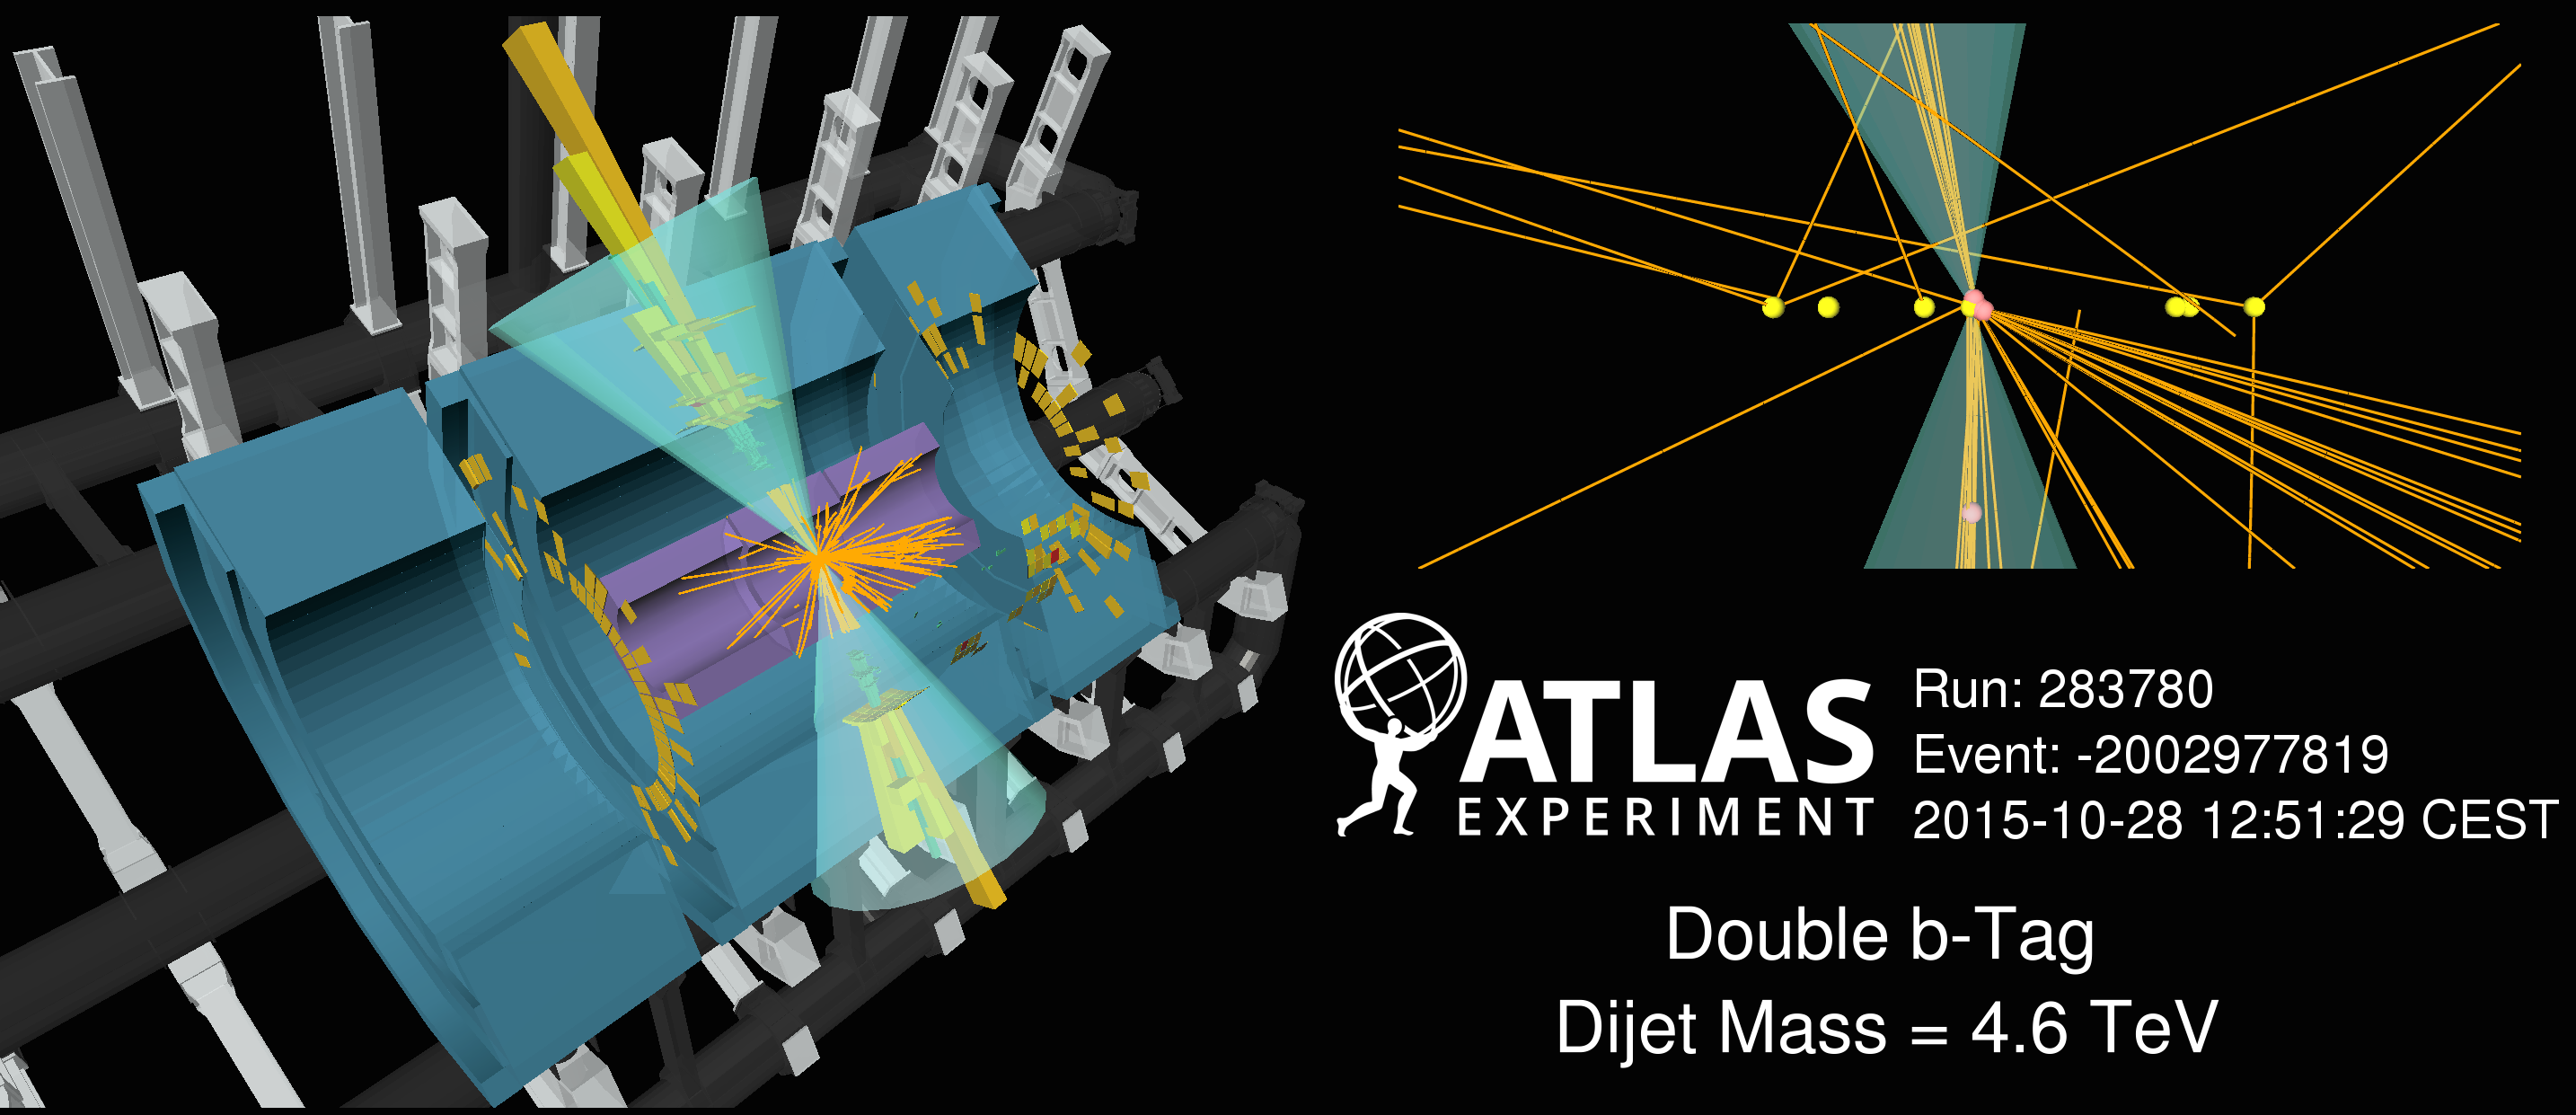
\includegraphics[width=0.95\linewidth, angle=0]{figs/Dibjet/Gen/evt-vp1_bb.png}}\\
   \subcaptionbox{$\geq$1 $b$-tag}{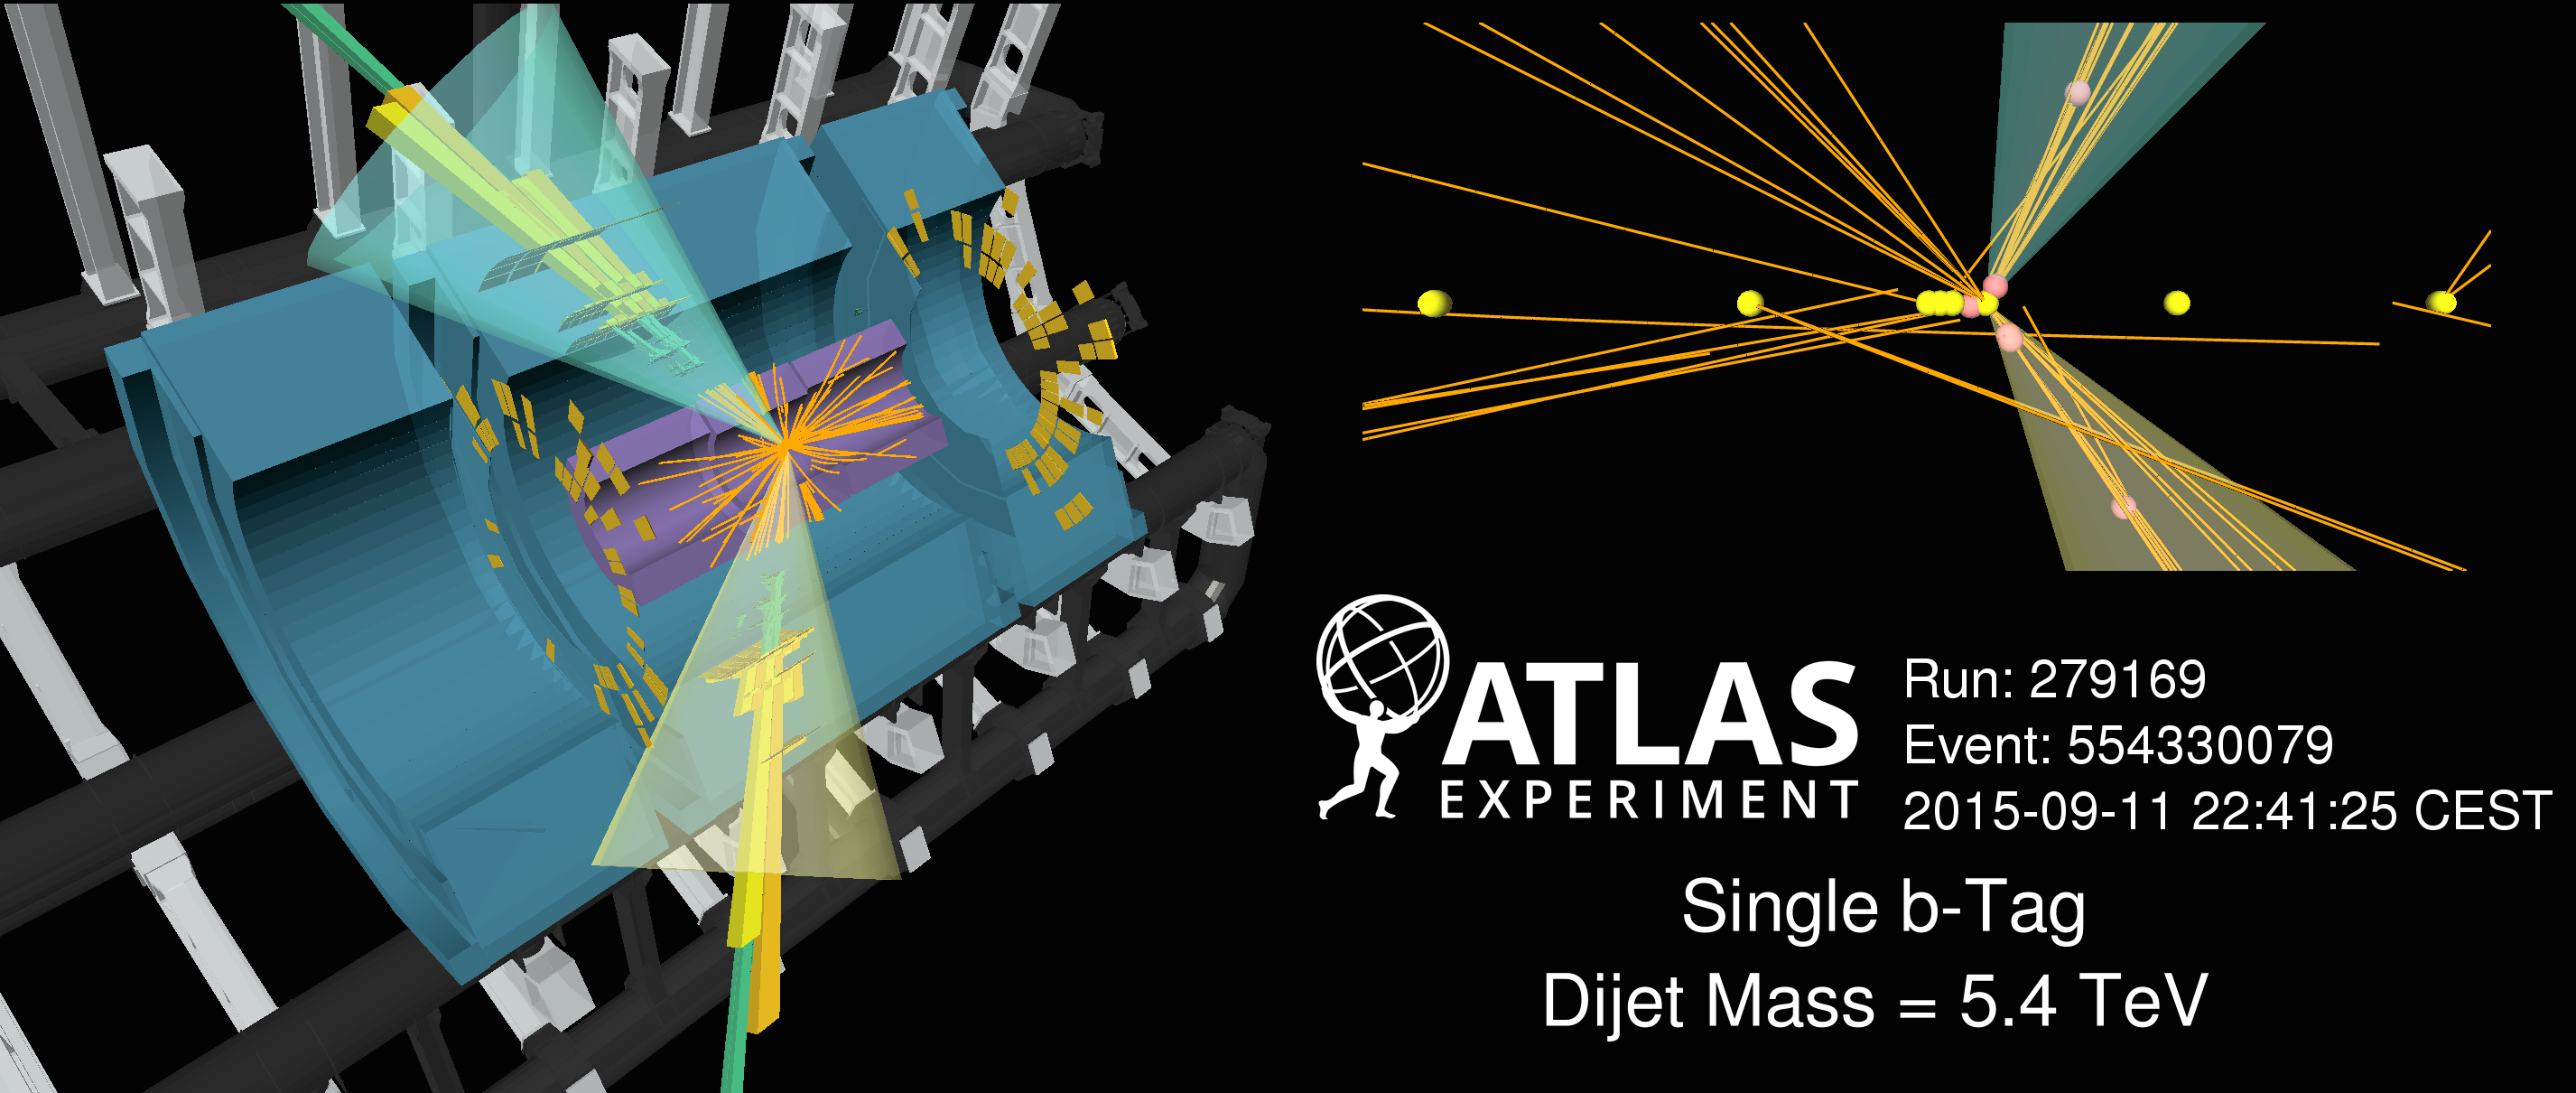
\includegraphics[width=0.95\linewidth, angle=0]{figs/Dibjet/Gen/evt-vp1_b.png}}
  \end{center}
  \caption
      {Event displays showing high~\mjj~events that pass the (a) 2 and (b) $\geq$1 $b$-tag di-$b$-jet event selection.
        The left section of the figures show a cut-away of the ATLAS detector;
        the inner detector is shown in purple, the hadronic calorimeter is shown in blue
        and the toroid magnet and supporting structure is shown in black and grey.
        The upper right section of the figures show a close-up view of the inner tracker in the $r-z$ plane.
        In both sections tracks inside the inner detector are shown in orange
        and energy deposits in the EM and hadronic calorimeter are shown in cyan and yellow respectively.
        The two leading jets formed are indicated by the cones, where a blue cone indicates that the jet has been
        $b$-tagged and a yellow cone shows that it has not.
        The yellow spheres show the primary vertex candidates and the red spheres show the secondary vertex candidates.
      }
  \label{fig:evt-vp1}
\end{figure}

With the event selection now defined,
the signal acceptance of the di-$b$-jet analysis is studied
to understand the performance of the analysis selection
and as an input to the limit-setting phase of the analysis.
The signal acceptance multiplied by trigger efficiency is defined as the 
the fraction of signal events that pass the analysis' trigger and event selection.
In addition, as $b$-tagging is a unique cut in our analysis relative to other dijet searches,
the event-tagging efficiency is also considered, which is defined as the fraction of events that pass
$b$-tagging cuts given that the event has passed all other aspects of the event selection.
Signal acceptance and event tagging efficiency are estimated using the
Monte-Carlo signal templates discussed in Section~\ref{sec:evt-s+b}.

For the \verb|Summer16+15| data-set event-selection;
Figure~\ref{fig:evt-ichep_acc}(a) shows the signal acceptance multiplied by trigger efficiency
for the $b^*$ and $Z'$ signal models
as a function of the simulated mass
in the case that $b$-tagging is applied and when it is not applied.
Figure~\ref{fig:evt-ichep_acc}(b) shows the event tagging efficiency
for the $b^*$ and $Z'$ for a range of simulated mass points
as a function of the reconstructed invariant mass,~\mjj.
In both plots the $b$-tagging category used is labelled in the legend.

There are a few features of the signal acceptance and tagging efficiency that can be commented on.
There is a reduced signal acceptance at lower values of simulated mass
because there is a low mass tail of the signal template which lies below the~\mjj~cut,
the tail is caused by a preference for low values of~\mjj~by the PDFs.
In addition, the event tagging efficiency decreases at high values of~\mjj~
due to a lower performance of $b$-tagging at high jet-\pT.
\textbf{LM Fix: Refer to high-pT~$b$-tagging, will be added to b-tag chapter}.
Finally, the $b^*$ quark has a similar tagging efficiency
as the $Z'$-boson in the $\geq$1 $b$-tag category at high~\mjj;
whilst naively one would expect that the $Z'$-boson should have a higher
event tagging efficiency as it decays to two $b$-quarks,
the gluon from the $b^*$ quark decay can split into a pair of lower~\pT~$b$-quarks
which can often be tagged leading to a similar tagging efficiency.

\begin{figure}[!ht]
  \begin{center}
    \captionsetup[subfigure]{aboveskip=0pt,justification=centering}
    \subcaptionbox{Signal acceptance multiplied \\by trigger efficiency}{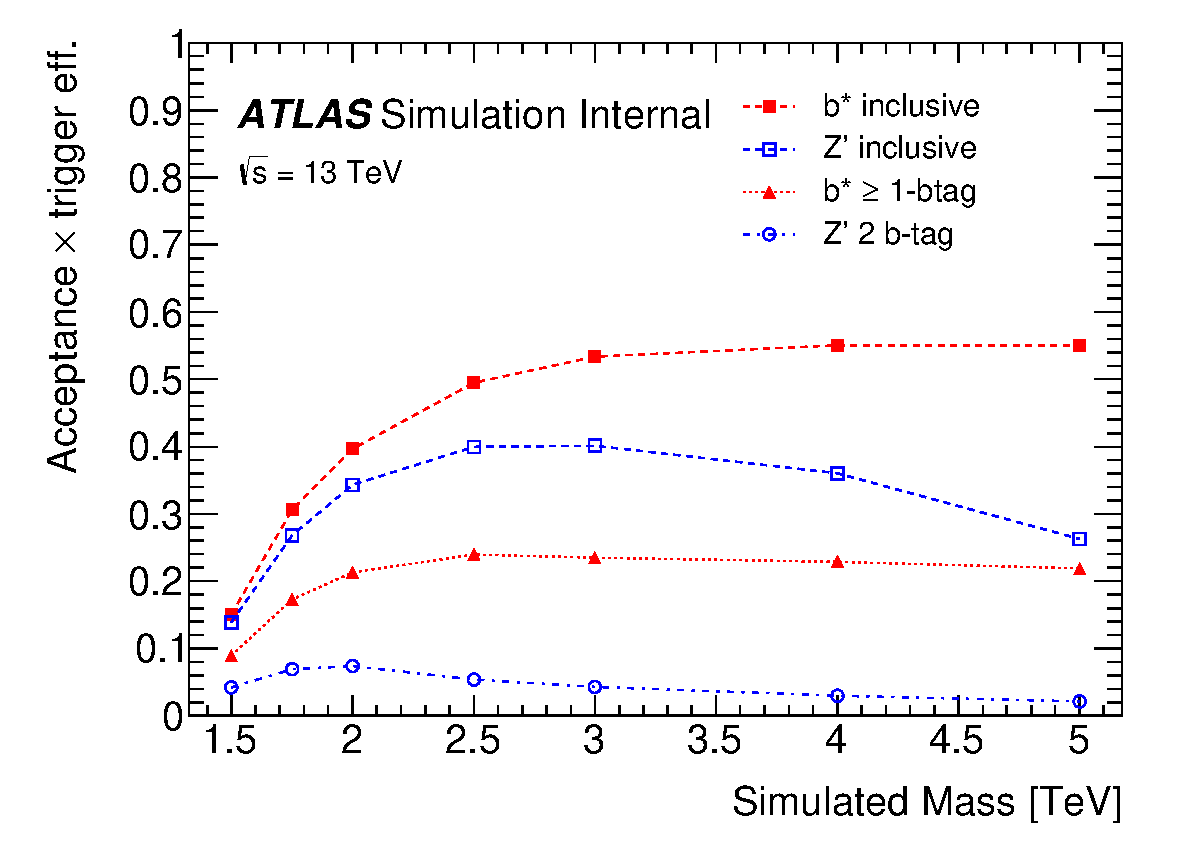
\includegraphics[width=0.48\linewidth, angle=0]{figs/Dibjet/ICHEP/evt-acc.pdf} }
    \subcaptionbox{Event tagging efficiency}{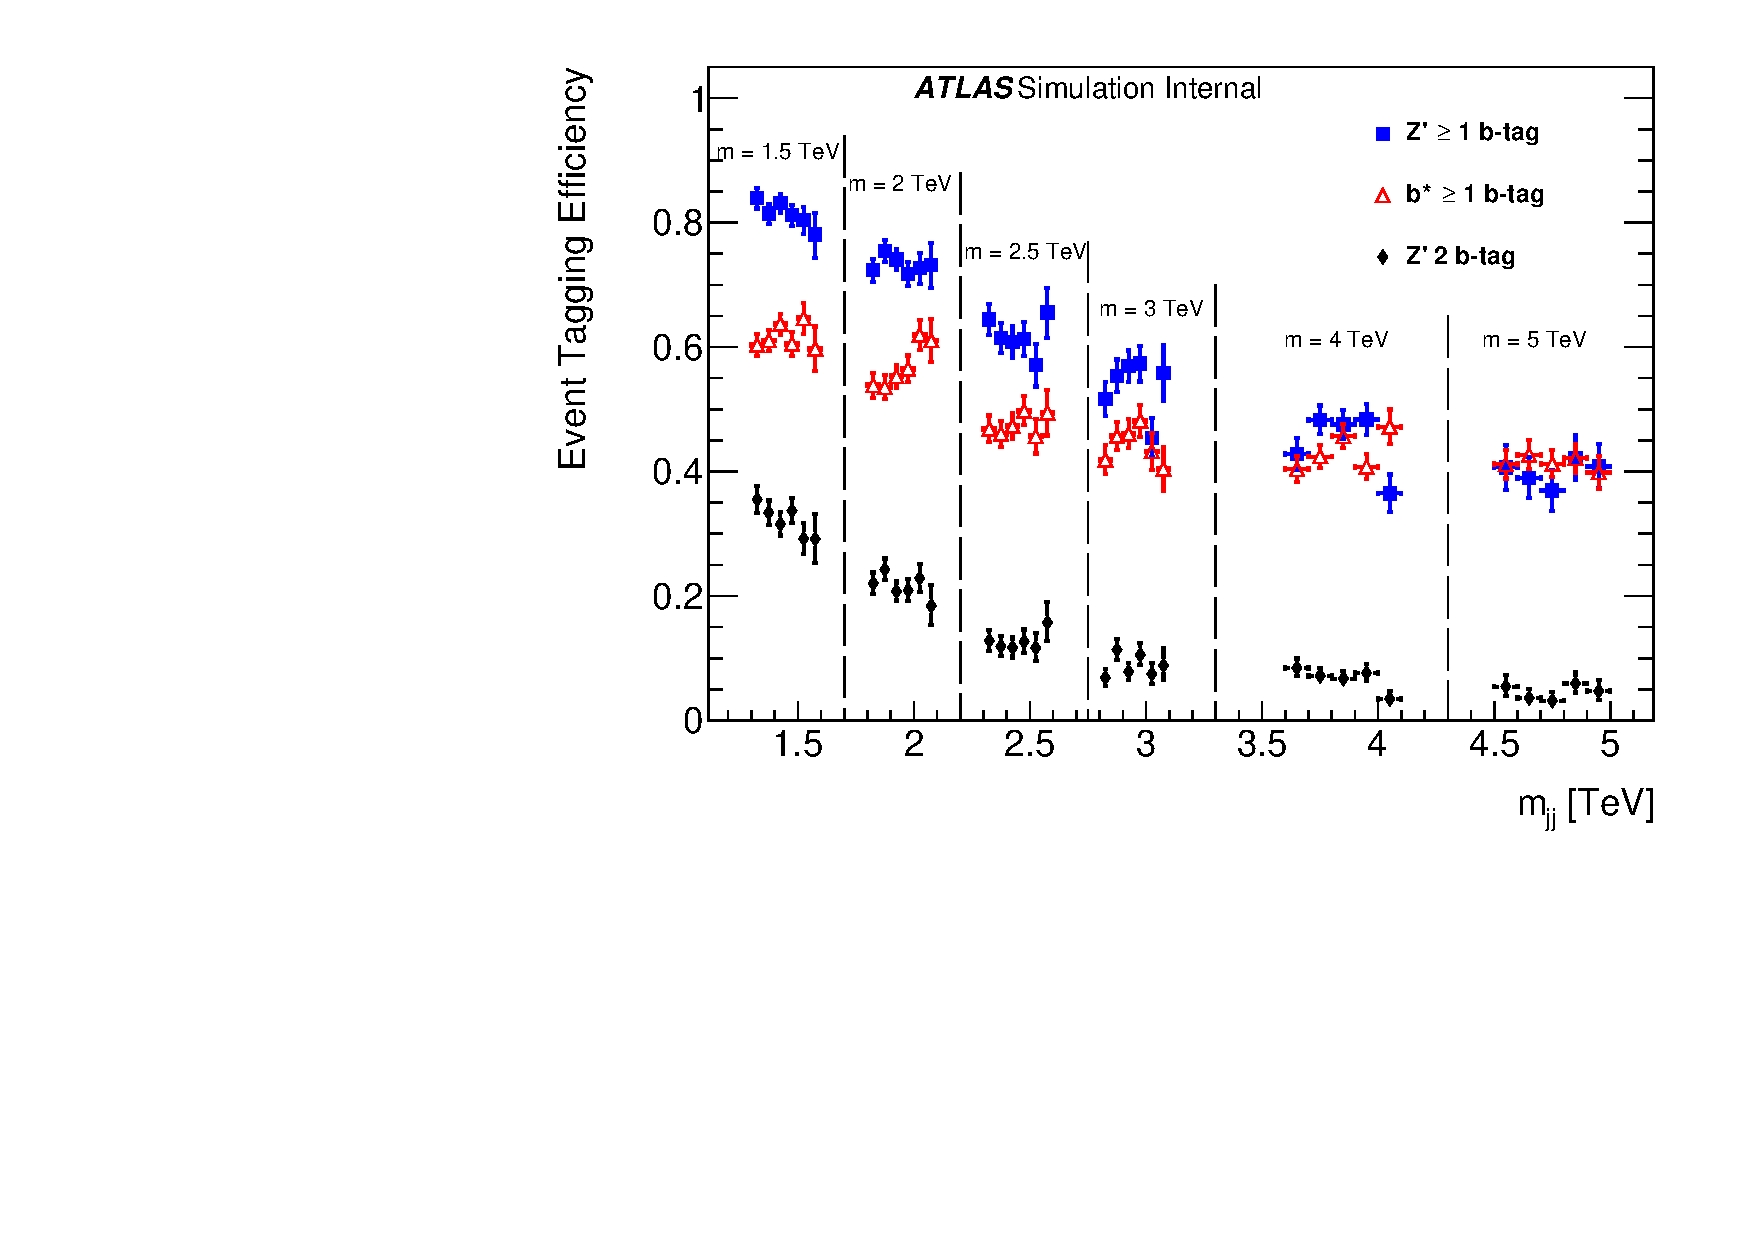
\includegraphics[width=0.48\linewidth, angle=0]{figs/Dibjet/ICHEP/evt-tagEff.pdf} }
  \end{center}
  \caption[Plots to show the acceptance of the \textit{Summer16+15} data-set event selection for the $b^*$ quark and $Z'$-boson signal models.
            Panel (a) shows the signal acceptance multiplied by trigger efficiency as a
            function of the simulated mass of the signal model, in the case where $b$-tagging has been applied and not.
            Panel (b) shows the event tagging efficiency as a function of the dijet invariant mass,~\mjj,
            for a range of simulated masses, $m$, as indicated on the plot.
            In both figures the $b$-tagging categories used are indicated in the legend.
            Details of the \textit{Summer16+15} data-set event selection are described in the text.]
          {Plots to show the acceptance of the \textit{Summer16+15} data-set event selection for the $b^*$ quark and $Z'$-boson signal models.
            Panel (a) shows the signal acceptance multiplied by trigger efficiency as a
            function of the simulated mass of the signal model, in the case where $b$-tagging has been applied and not.
            Panel (b) shows the event tagging efficiency as a function of the dijet invariant mass,~\mjj,
            for a range of simulated masses, $m$, as indicated on the plot.
            In both figures the $b$-tagging categories used are indicated in the legend.
            Details of the \textit{Summer16+15} data-set event selection are described in the text.
            Figures taken from~\cite{dibjet-ichep_conf}.} 
  \label{fig:evt-ichep_acc}
\end{figure}
